%%%%%%%%%%%%%%%%%%%%%%%%%%%%%% -*- Mode: Latex -*- %%%%%%%%%%%%%%%%%%%%%%%%%%%%
%% uhtest.tex -- 
%% Author          : Robert Brewer
%% Created On      : Wed Sep 30 16:08:49 1998
%% Last Modified By: Robert Brewer
%% Last Modified On: Mon Oct  5 16:17:16 1998
%% RCS: $Id: uhtest.tex,v 1.2 1998/10/06 02:04:56 rbrewer Exp rbrewer $
%%%%%%%%%%%%%%%%%%%%%%%%%%%%%%%%%%%%%%%%%%%%%%%%%%%%%%%%%%%%%%%%%%%%%%%%%%%%%%%
%%   Copyright (C) 1998 Robert Brewer
%%%%%%%%%%%%%%%%%%%%%%%%%%%%%%%%%%%%%%%%%%%%%%%%%%%%%%%%%%%%%%%%%%%%%%%%%%%%%%%

%!!!!!!!!!!!!!!!!!!!!!!!!!!!!!!!!!!!!!!!!!!!!!!!!!!!!!!!!!!!!!!!!!!!!!!!!!!!!!!
%!NOTE: This example file has been prepared according to the University of
%!      Hawaii Style & Policy Manual for Theses and Dissertations dated
%!      "Revised February 1998". If you have one with a later date, you may
%!      need to make revisions to this document as well. In any event, making
%!      sure your thesis complies with Graduate Division guidelines is
%!      ultimately your responsibility. Caveat LaTeXtor. :)
%!!!!!!!!!!!!!!!!!!!!!!!!!!!!!!!!!!!!!!!!!!!!!!!!!!!!!!!!!!!!!!!!!!!!!!!!!!!!!!

%% The options are (you can only choose one from each group):
%%
%% 10pt, 11pt, 12pt: chooses the point size for the document. "11ot" is the
%%                   default.
%%
%% oneside, twoside: whether you want your document onesided or twosided. Note
%%                   that twosided is not guaranteed to work, and style
%%                   guidelines prohibit double sided printouts on final
%%                   copy. "oneside" is the default.
%%
%% draft, final: when printing drafts you can save a lot of paper by using the
%%               "draft" option. It switches to single spacing, displays overful
%%               hboxes with a black box, prints a version number on title page 
%%               and omits signature page. Of course for the final copy make
%%               sure to use the "final" option! "final" is the default.
%%
%% cm, times, palatino, newcent, bookman: switches between different font
%%                                        sets. "cm" is the Computer Modern
%%                                        font (TeX's default), the rest are
%%                                        PostScript fonts. "times" is the
%%                                        default.
%%
%% thesis, dissertation: switches between the style for a master's thesis and a 
%%                       Ph.D. dissertation. The differences are fairly minor
%%                       and limited to the front matter. "thesis" is the
%%                       default.
%%
%% actual, proposal: switches between actual document and proposal mode. In
%%                   proposal mode: the title page is simplified, the
%%                   version number is always printed, and the signature page
%%                   is omitted.
%%
\documentclass[11pt]{article}
\usepackage[final]{graphicx}
\usepackage{times}

%% Make subsubsections numbered and included in ToC
\setcounter{secnumdepth}{3}
\setcounter{tocdepth}{3}

%% URLs
\usepackage{url}
\usepackage[colorlinks, bookmarks=true]{hyperref}

%% Define a new 'smallurl' style for the package that will use a smaller font.
\makeatletter
\def\url@smallurlstyle{%
  \@ifundefined{selectfont}{\def\UrlFont{\sf}}{\def\UrlFont{\small\ttfamily}}}
\makeatother
%% Now actually use the newly defined style.
\urlstyle{smallurl}

%% CO2 
\usepackage{xspace}
\newcommand{\COtwo}{CO\ensuremath{_2}\xspace}

%% Make margins less ridiculous
\usepackage{fullpage}

\usepackage{floatflt}
\usepackage{wrapfig}

%% Since I'm using the LaTeX Makefile that uses dvips, I need this
%% package to make URLs break nicely
\usepackage{breakurl}

\usepackage{graphicx}

%%% Declarations for Front Matter. Capitalize all of these values
%%% "normally". This allows the document class to format them properly.
%% Full title of thesis or dissertation, capitalized like a title should be.
\title{Design, Implementation, and Initial Evaluation of OPQBox: A low-cost device for crowdsourced power quality monitoring}
%% Your name, capitalized normally. Do not include any titles like Dr.
\author{Sergey Negrashov}


%%% End of preamble
\begin{document}
\maketitle


%%% Bring in the abstract section from external file
%%%%%%%%%%%%%%%%%%%%%%%%%%%%%% -*- Mode: Latex -*- %%%%%%%%%%%%%%%%%%%%%%%%%%%%
%% uhtest-abstract.tex -- 
%% Author          : Robert Brewer
%% Created On      : Fri Oct  2 16:30:18 1998
%% Last Modified By: Robert Brewer
%% Last Modified On: Fri Oct  2 16:30:25 1998
%% RCS: $Id: uhtest-abstract.tex,v 1.1 1998/10/06 02:06:30 rbrewer Exp $
%%%%%%%%%%%%%%%%%%%%%%%%%%%%%%%%%%%%%%%%%%%%%%%%%%%%%%%%%%%%%%%%%%%%%%%%%%%%%%%
%%   Copyright (C) 1998 Robert Brewer
%%%%%%%%%%%%%%%%%%%%%%%%%%%%%%%%%%%%%%%%%%%%%%%%%%%%%%%%%%%%%%%%%%%%%%%%%%%%%%%
%% 

\begin{abstract}
The face of power distribution has changed rapidly over the last several decades.
Modern grids are evolving to accommodate distributed power generation, and  highly variable loads.
Furthermore as the devices we use every day become more electronically complex,
they become increasingly more sensitive to power quality problems. A distributed 
power quality monitoring systems have been shown to provide real-time insight on the
status of the power grid and even pinpoint the origin of the power disturbance. \cite{fnet_defence}
Oahu's isolated power grid combined with high penetration of distributed renewable energy generators create perfect
conditions for deploying of such a network. Over the last three months we have been collecting power
quality data from several locations of the island as a pilot study for a larger monitoring system.
This papers describes our methodology, hardware and software design and presents a preliminary analysis
of the data we collected so far. Lastly this paper presents the next generation of the power quality monitor
to be used in an island wide monitoring system.
\end{abstract}


%%% Generate table of contents
\tableofcontents
\newpage
%%% Generate list of figures
\listoffigures


%\normalsize
%%% Bring in the body of the thesis from external file
%%%%%%%%%%%%%%%%%%%%%%%%%%%%%% -*- Mode: Latex -*- %%%%%%%%%%%%%%%%%%%%%%%%%%%%
%% uhtest-body.tex -- 
%% Author          : Robert Brewer
%% Created On      : Fri Oct  2 16:30:37 1998
%% Last Modified By: Robert Brewer
%% Last Modified On: Mon Oct  5 16:01:29 1998
%% RCS: $Id: uhtest-body.tex,v 1.1 1998/10/06 02:07:14 rbrewer Exp $
%%%%%%%%%%%%%%%%%%%%%%%%%%%%%%%%%%%%%%%%%%%%%%%%%%%%%%%%%%%%%%%%%%%%%%%%%%%%%%%
%%   Copyright (C) 1998 Robert Brewer
%%%%%%%%%%%%%%%%%%%%%%%%%%%%%%%%%%%%%%%%%%%%%%%%%%%%%%%%%%%%%%%%%%%%%%%%%%%%%%%
%% 

\section{Introduction}

The face of a modern power grid has changed dramatically over the last few decades. A grid based upon a few centralized power generators has given way to a composite architecture, where distributed renewable sources work in synergy with the municipal power plants. This trend is accelerating as renewable energy generators, such as PV and wind  turbines become cheaper and more efficient. Unfortunately, most renewable sources are not able to provide ``firm'' (i.e. consistent, predictable, and controllable)  power. This has an adverse effect on the grid stability as has been previously demonstrated.\cite{pq_effect1}\cite{pq_effect2}

Oahu's power grid provides an ideal testbed for a power monitoring study. It's a small isolated system with high penetration of renewable power generators. Furthermore, the Oahu power grid has been been slow to adjust to distributed generation. New PV and wind generators now undergo careful scrutiny by the utility, in an attempts minimize the adverse effects on the grid. There is a need for additional data regarding the quality of power generated on the island, and whether or not there exists correlations  to environmental factors.

Over the last three months the Open Power Quality group has been collecting $V_{rms}$ and $f_{utility}$ data across five different locations as part of a pilot study for a larger scale deployment. This paper describes the prototype system, presents an initial analysis of the collected data, and finally presents the next generation of our power quality meter designed for island wide deployment. First however, we must describe the metrics and background of power quality measurements.

\subsection{Power grids and power quality}

Modern power grids provide a fixed AC frequency at a set voltage. For United States this amounts to a $60Hz$, and $120V_{rms}$. Power quality on the voltage side is the  measure of the frequency composition and RMS of the voltage across several grid cycles. An ontology of power quality events and classification methods has been presented across several publications.\cite{pq_onto1} \cite{pq_class} For the purpose of this study we focus on rudimentary metrics for power quality:

\begin{enumerate}
\item Voltage fluctuations($V_{rms}$).
\item Utility frequency($f_{utility}$).
\end{enumerate}

Root mean square of a voltage is a useful tool for analyzing voltage time series. It measures the equivalent DC voltage for a time varying signal. RMS Voltage in the discrete domain can be calculated via:
\begin{equation}
\label{eq:rms}
\centering
V_{rms} = \sqrt{\frac{1}{N} \sum_{0}^{n}{V_{n}^2}}
\end{equation}
Variations in the RMS can lead to conditions known as sags/brownouts and swells. A voltage sag is a 10\%-80\% drop in the power line voltage ranging in duration from half of a grid cycle to one minute. A brownout is a sag lasting longer then a minute. The ITIC curve is the industry standard for evaluating the severity of voltage sags for 120V, 60Hz grids. However the ITIC curve does not take into account the geographical area affected by the disturbance.

Another useful metric for studying power quality is the utility frequency($f_{utility}$). Utility frequency is the fundamental frequency of AC power distribution. There are several methods of measuring the utility frequency from discrete voltage measurement. For example, the voltage signal can be analyzed in frequency domain, where fitting of the maxima can be used to extract the fundamental frequency. Waveform can be analyzed in time domain via fitting or a phase locked loop. Some power quality algorithms employ wavelet transforms to detect variation in the utility frequency.\cite{pq_class}

\subsection{Measuring Grid Health on a Residential Scale}
On Oahu, the utility company monitors the state of the grid down to the substation level. This means that they generally have no situational awareness of power quality at consumer level. Furthermore, they do not report much information regarding power quality. The lowest granularity event they are required to disclose is a power outage lasting longer then 3 minutes. In order to gain insight into the health of the power grid at the residential level, a distributed real-time power quality monitoring system is required. Such a system would monitor the line voltage and frequency below the substation level and combine this data to produce a meaningful picture of the grid health. In order for a power quality monitoring system to be useful it must fulfill several criteria:
\begin{itemize}
\item \textbf{Availability.} Power grids operate without interruption, and so must the monitoring system.

\item \textbf{Filtering.} High end commercial power quality measurement systems sample 256 or more data point for every grid cycle, using 16bit resolution. This results in the raw data rate of 400kb/s per device. The logical choice for data aggregation is TCP/IP. Residential cable  subscription provides upload speeds the order of 1Mbps, and so transport of uncomressed and unfiltered waveforms would significantly degrade the quality of Internet service. Furthermore, 100 devices would produce an aggregate bandwidth of 40Mbps, limiting the scalability of such a system. Finally, raw data which exhibits normal grid operation is not interesting, and can be reduced to $V_{rms}$ voltage and frequency. In order to overcome these problems, voltage waveforms should be preprocessed by the measurement device. This way, power quality events such as transients can be sent over to the aggregation service in their
raw state state. The rest of the data can be reduced to a few fundamental values, such as $f_{utility}$ and $V_{rms}$ over a sliding window, which greatly reducing the required bandwidth.

\item \textbf{Density.} Ideally a power quality monitoring system would have several meters for every group of consumers connected to a given
substation. Consumer level power quality can be affected by a multitude of local sources unrelated to the overall grid health. For example, we demonstrated that 
a heating coil, such as a water heater or even an electric kettle, can cause a voltage sag while powered. On the other hand large inductive loads, such as air conditioners, 
can cause a large transient due to the inrush current requirements. By having several units connected under the same substation it is possible to filter the noise generated
by the regular activities of a consumer, and evaluate the overall grid status instead.

\item \textbf{Synchronization.} Temporal synchronization is required to separate local events from grid wide disturbances.  NTP and GPS are common choices for sensor network synchronization. 

\end{itemize}

Devices that measure power quality are known as power quality meters. These devices monitor the voltage and sometimes current provided by the grid, and analyze it according to common power quality metrics. Most publicly available power quality meters fall into two categories:

\begin{itemize}
\item Professional grade such as National Instruments\textregistered 862001. \cite{NI-device} These devices are generally used by the utility companies, and power system engineers. They combine high accuracy measurement electronics, with fast digital signal processors in order to provide detection and classification of power quality events.These devices allow for unparalleled connectivity from WIFI, to CAN bus, and power line communications.  Unfortunately the cost of these meters prohibits their use in a distributed grid study where several dozen, or even hundreds of devices are required.
\item Consumer grade such as AC Scout\textregistered. \cite{ACScout} These devices are simple voltage line monitors. They provide adequate power quality measurements to give homeowners insight into the state of their electrical wiring and the health of the grid as a whole. Unfortunately these devices leave much to be desired when it comes to communication. Generally they offer no connectivity beyond external storage. This makes them unattractive for a distributed real-time monitoring systems.
\end{itemize}

Several power quality meters designed for distributed monitoring exist in academic and industrial installations.\cite{fnet_main} Unfortunately these devices are not available for purchase, and some require an NDA to obtain.

\section{OPQ: cloud based power quality monitoring network.}

Over the last nine months, the Open Power Quality project \cite{OPQ} has developed an in-house prototype power quality meter (OPQBox \cite{OPQBox1Repository}) with wifi/ethernet connectivity that is suitable for wide-scale deployment. Furthermore, we developed a cloud based aggregation system (OPQhub \cite{OPQHubRepository}) designed for aggregating, analyzing, and displaying grid status. Over the last three months we have collected $V_{rms}$ and $f_{utility}$ data across five different locations as part of a pilot study for a larger deployment. This section describes the design of the power quality meter OPQBox1.

\subsection{OPQBox1: A Prototype Power Quality Monitor.}

OPQBox1 is an in-house developed power quality monitor, specifically designed for distributed use. It is capable of continuous 4Ksps 16Bit measurement of the line voltage, along with
on-board filtering and processing. The block diagram for this device is shown below:

\begin{figure}[h!]
\centering
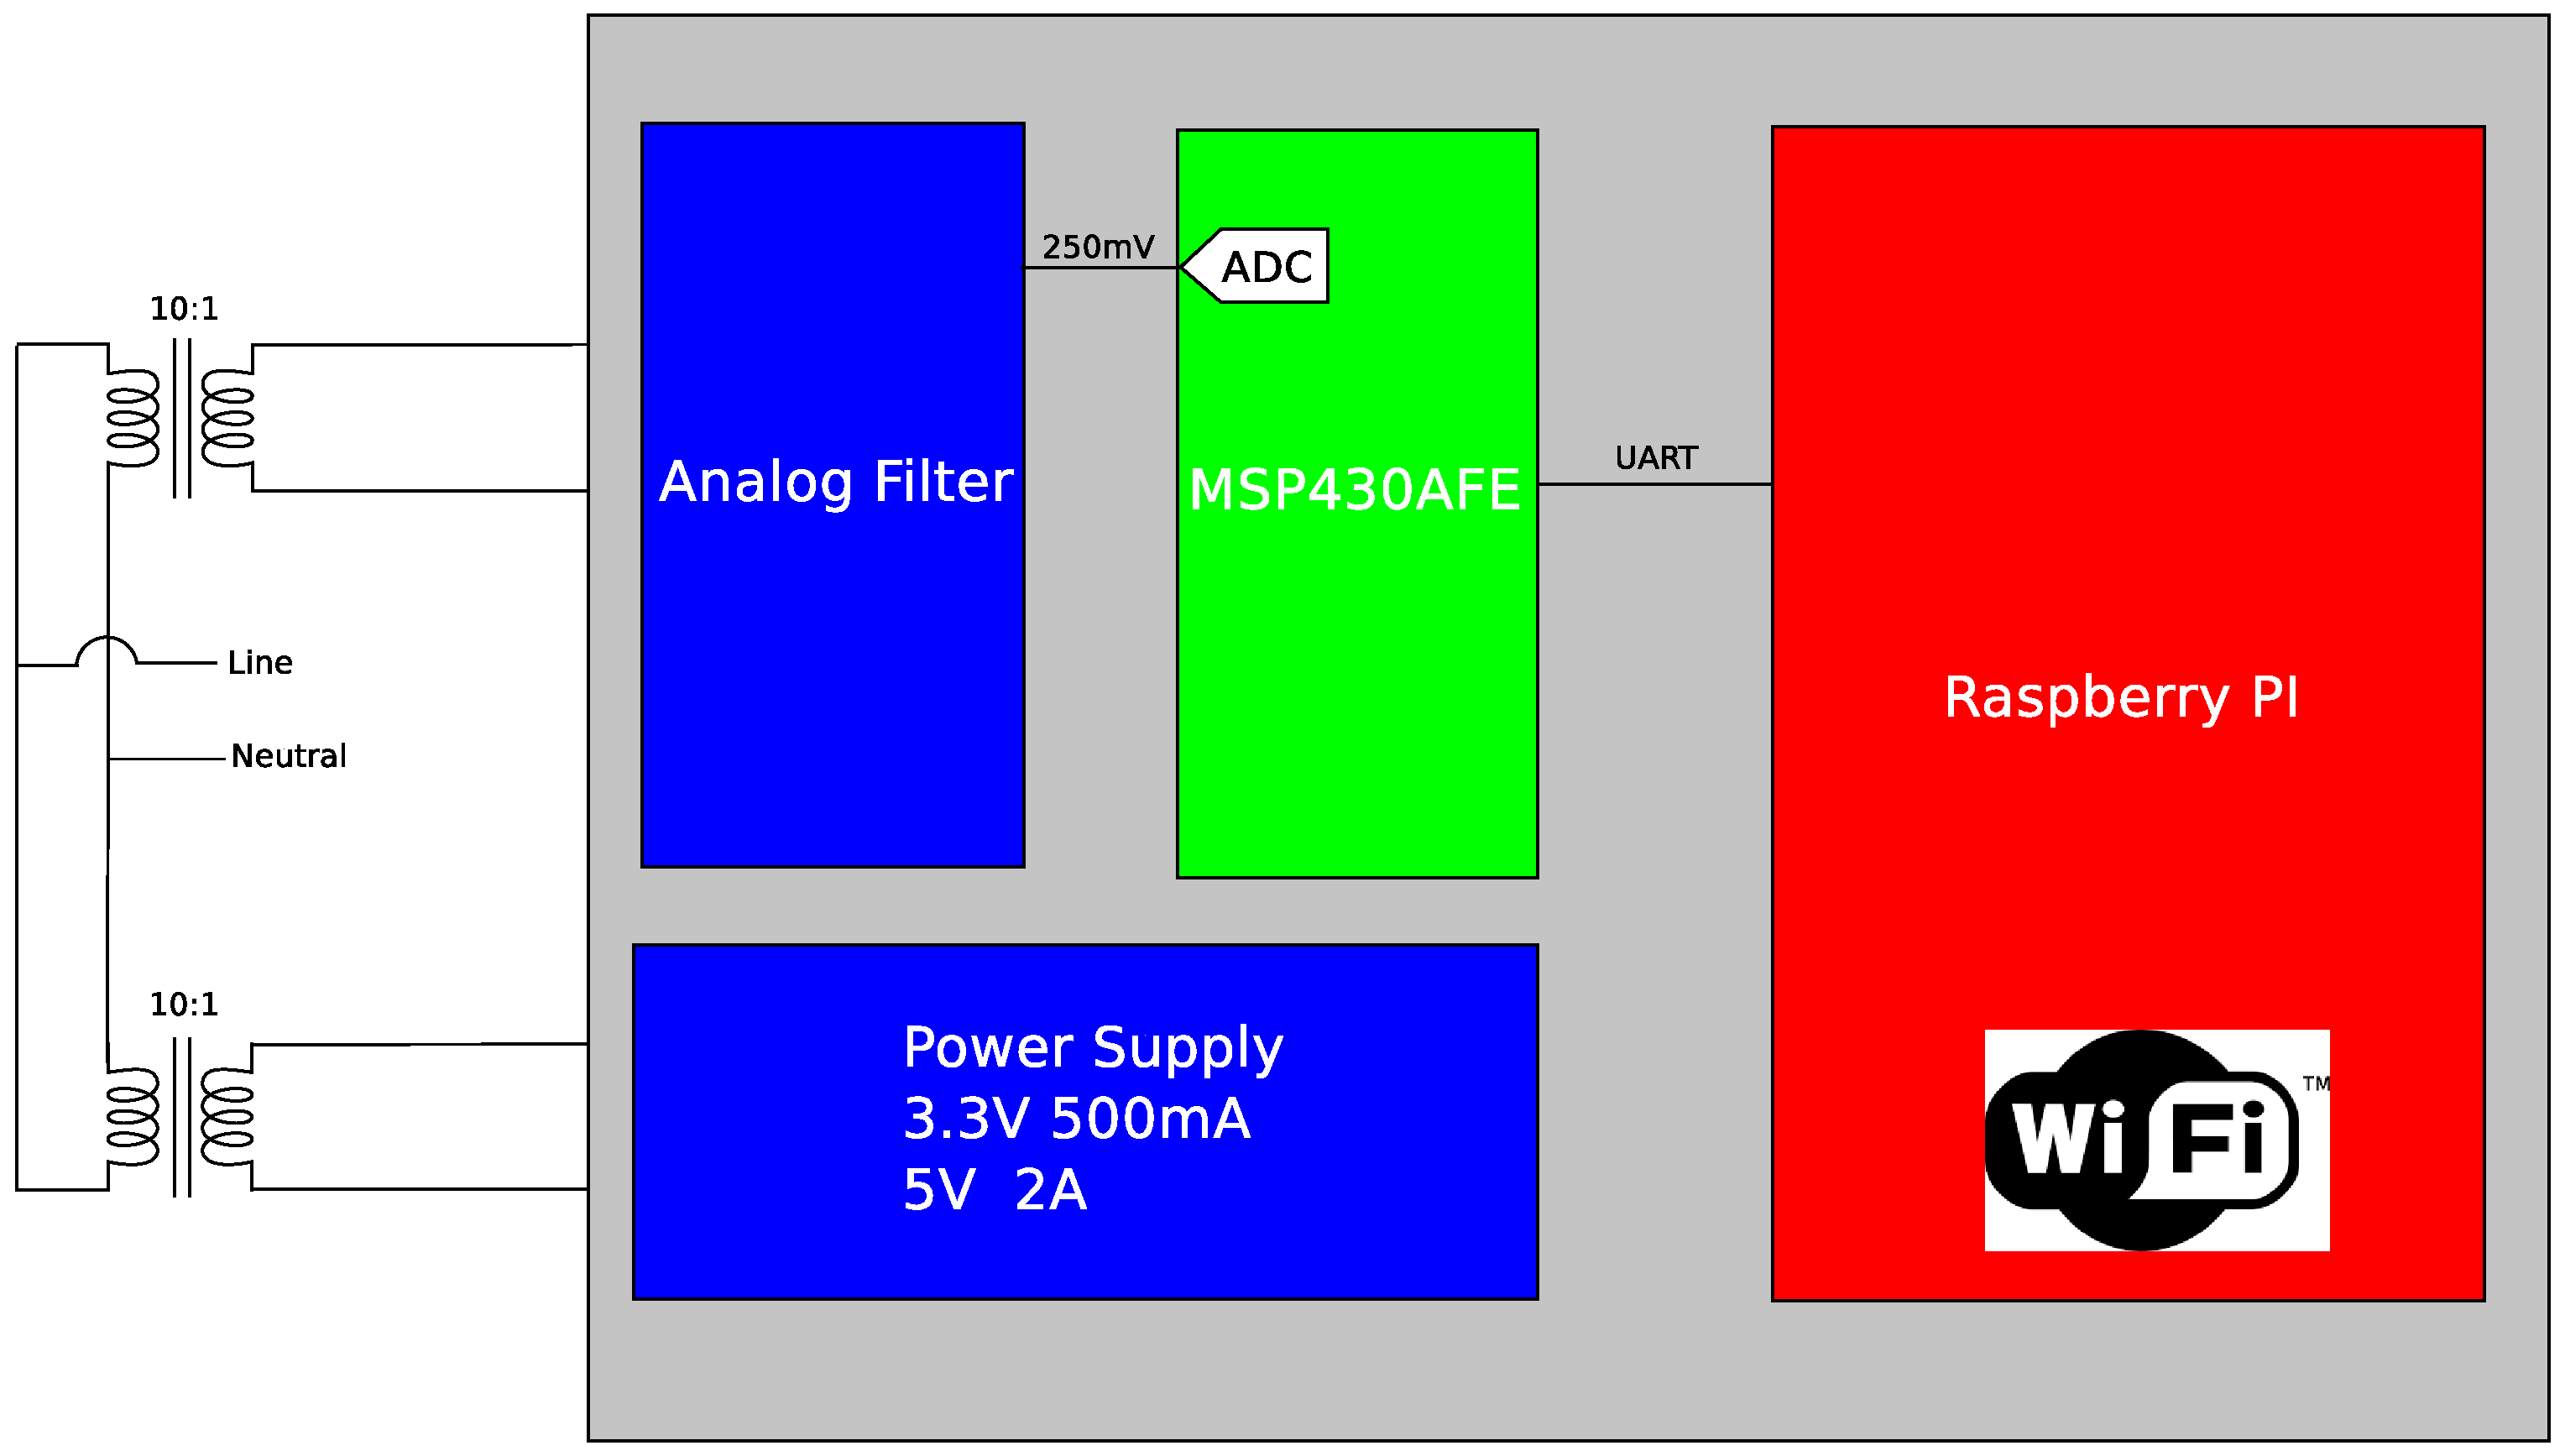
\includegraphics[width=0.7\textwidth]{img/OHM1Block.eps}
\caption{OPQBox Block Diagram}
\end{figure}

At the heart of the device is the MSP430AFE integrated circuit by Texas Instruments \textregistered. \cite{MSP430AFE} This innovative device combines a 24bit $\Sigma\Delta$ analog to digital converter(ADC), along with an MSP430 CPU core. MSP430 CPU controls the hard real-time acquisition tasks, however with the peak of 8 MIPS, 512 bytes of RAM and no floating point unit, this device is not capable to analyze the data it is gathering on its own. The soft real-time analysis is performed on a Raspberry PI single board computer (SBC). \cite{RaspberryPI} Raspberry Pi is a readily available SBC based on an 800Mhz ARM11 SOC by Broadcom\textregistered. It features a high variety of digital peripherals, fast CPU with FPU and 512MB of memory. Furthermore this SBC is well supported by the Linux kernel and user land, with most drivers being open source and highly stable. Raspberry PI reads and accumulates the ADC values generated by the MSP430 via a serial link. Once 4000 samples, or 1 second worth of data have been gathered, SBC performs rudimentary analysis and send power quality events, and trends to the cloud via WIFI. Synchronization between devices is accomplished via disciplining the local clock via NTP. While the analysis on the level of temporal synchronization is still being performed, it has been shown to be under 40ms device-to-device.

\subsection{Acquisition design.}

In order to measure the line voltage, it must first be scaled down to the ADC input range. This is performed in two stages. First a 10:1 transformer which isolates the circuit from the mains, as well as steps down the $120V_{rms}$ to $12V_{rms}$. Next, a passive network further scales the $12V_{rms}$ input to $200mV_{pp}$. Finally, the MSP430AFE digitizes the signal via a 24bit $\Sigma\Delta$ ADC. ADC modulation frequency is set to 1Msps with the oversampling rate of 256 to achieve the 24bit resolution and 4kHz sampling rate. The state machine of the MSP430 firmware is shown below. At startup, the MSP430 sets up the ADC, internal clocking, and the UART interfaces. Once the setup is finished, the firmware enters the IDLE state, putting the CPU in a low power mode. It remains in this mode until one of the following three conditions are met:

\begin{enumerate}
\item \textbf{Reset line is pulled low/Power cycle.} In this case the CPU will configure all of the peripherals, and enter the IDLE state once more.
\item \textbf{ADC interrupt fires.} This signifies that a new ADC sample is ready.
\item \textbf{WR Flag is pulled low.} This asserts that the Raspberry PI is ready to receive voltage samples.
\end{enumerate}

\begin{figure}[h!]
\centering
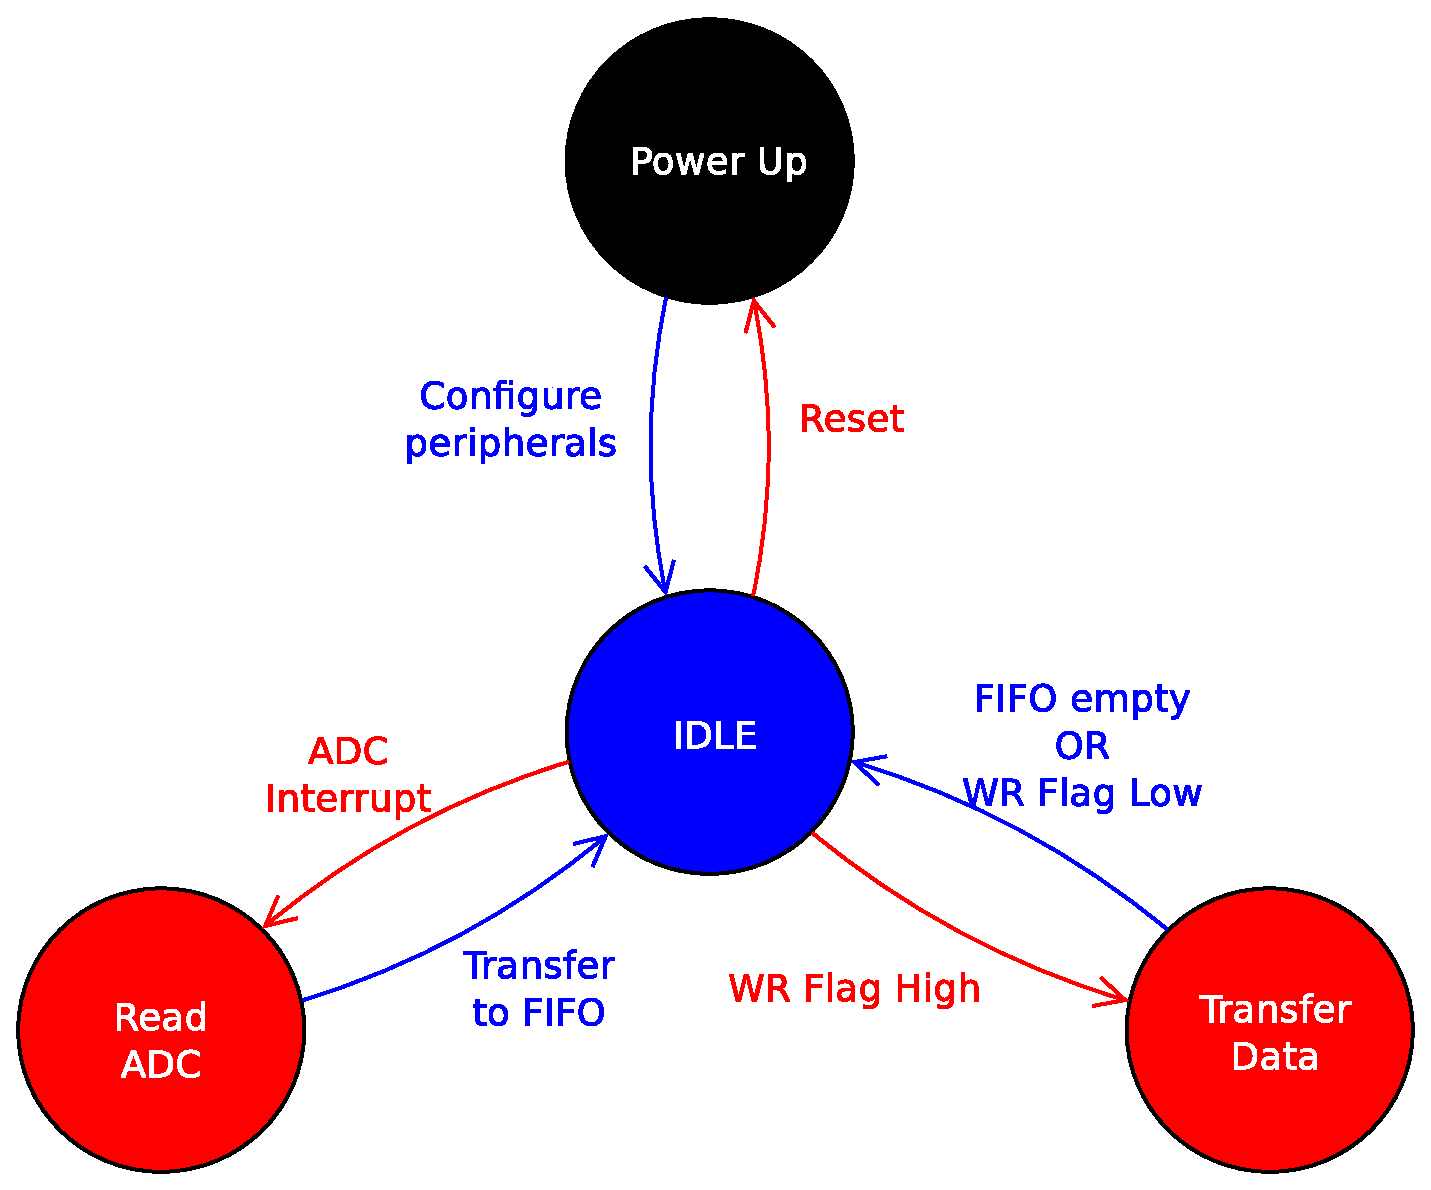
\includegraphics[width=0.5\textwidth]{img/MSP430StateMachine.eps}
\caption{MSP430 State Machine}
\end{figure}

The ADC is operating in free-running mode, meaning that the conversion timing is controlled via hardware. Once the conversion is complete, a system interrupt notifies the CPU. In order to remove the hard real-time constraint for the Raspberry PI, the MSP430 CPU stores the ADC readings in an 85 sample FIFO. This FIFO, implemented as a circular buffer,  allows the Raspberry PI to receive data at non-regular intervals. This is important since the Raspberry PI is running a non real-time operating system. If the FIFO is full, the oldest sample is dropped from FIFO. Unfortunately there is no mechanism to inform the Raspberry PI of an overflow in OPQBox1. This will be remedied in the next generation design of the meter. See section \ref{chap:further} for more details on the next generation device design.

Communication between the Raspberry PI and the MSP430AFE is performed via UART with the addition of a WR line. When the WR line is pulled low, a level triggered interrupt notifies the MSP430 CPU that the PI is ready for more data. The data is transfered via UART running at 230400bps.

\subsection{Data filtering and local analysis}

The Raspberry PI is responsible for selecting events which deviate from the steady state condition. In our case, steady state is a sinusoid with a set frequency and amplitude. Acquisition and processing is performed in five steps:

\begin{enumerate}
\item Acquisition.
\item Frequency calculation.
\item RMS calculation.
\item Event Filter.
\item Communication.
\end{enumerate}

The acquisition step accumulates a 4000 sample window, and passes it on for processing. In order to align the data during aggregation, the Raspberry PI generates a time-stamp for each window. Next, the fundamental frequency of the waveform is computed. In order to do that, a Fourier transform of the sample window is performed. Six points surrounding the largest FFT peak are selected, and fitted with a Gaussian in order to extract the true utility frequency as shown in figure \ref{fig:fit}. Finally,  $V_{rms}$ is computed for each window according to the equation \ref{eq:rms}.  Only complete half-periods are included in $V_{rms}$ calculation, and the leading and trailing samples are pruned. 

\begin{figure}[h!]
\begin{center}
\label{fig:fit}
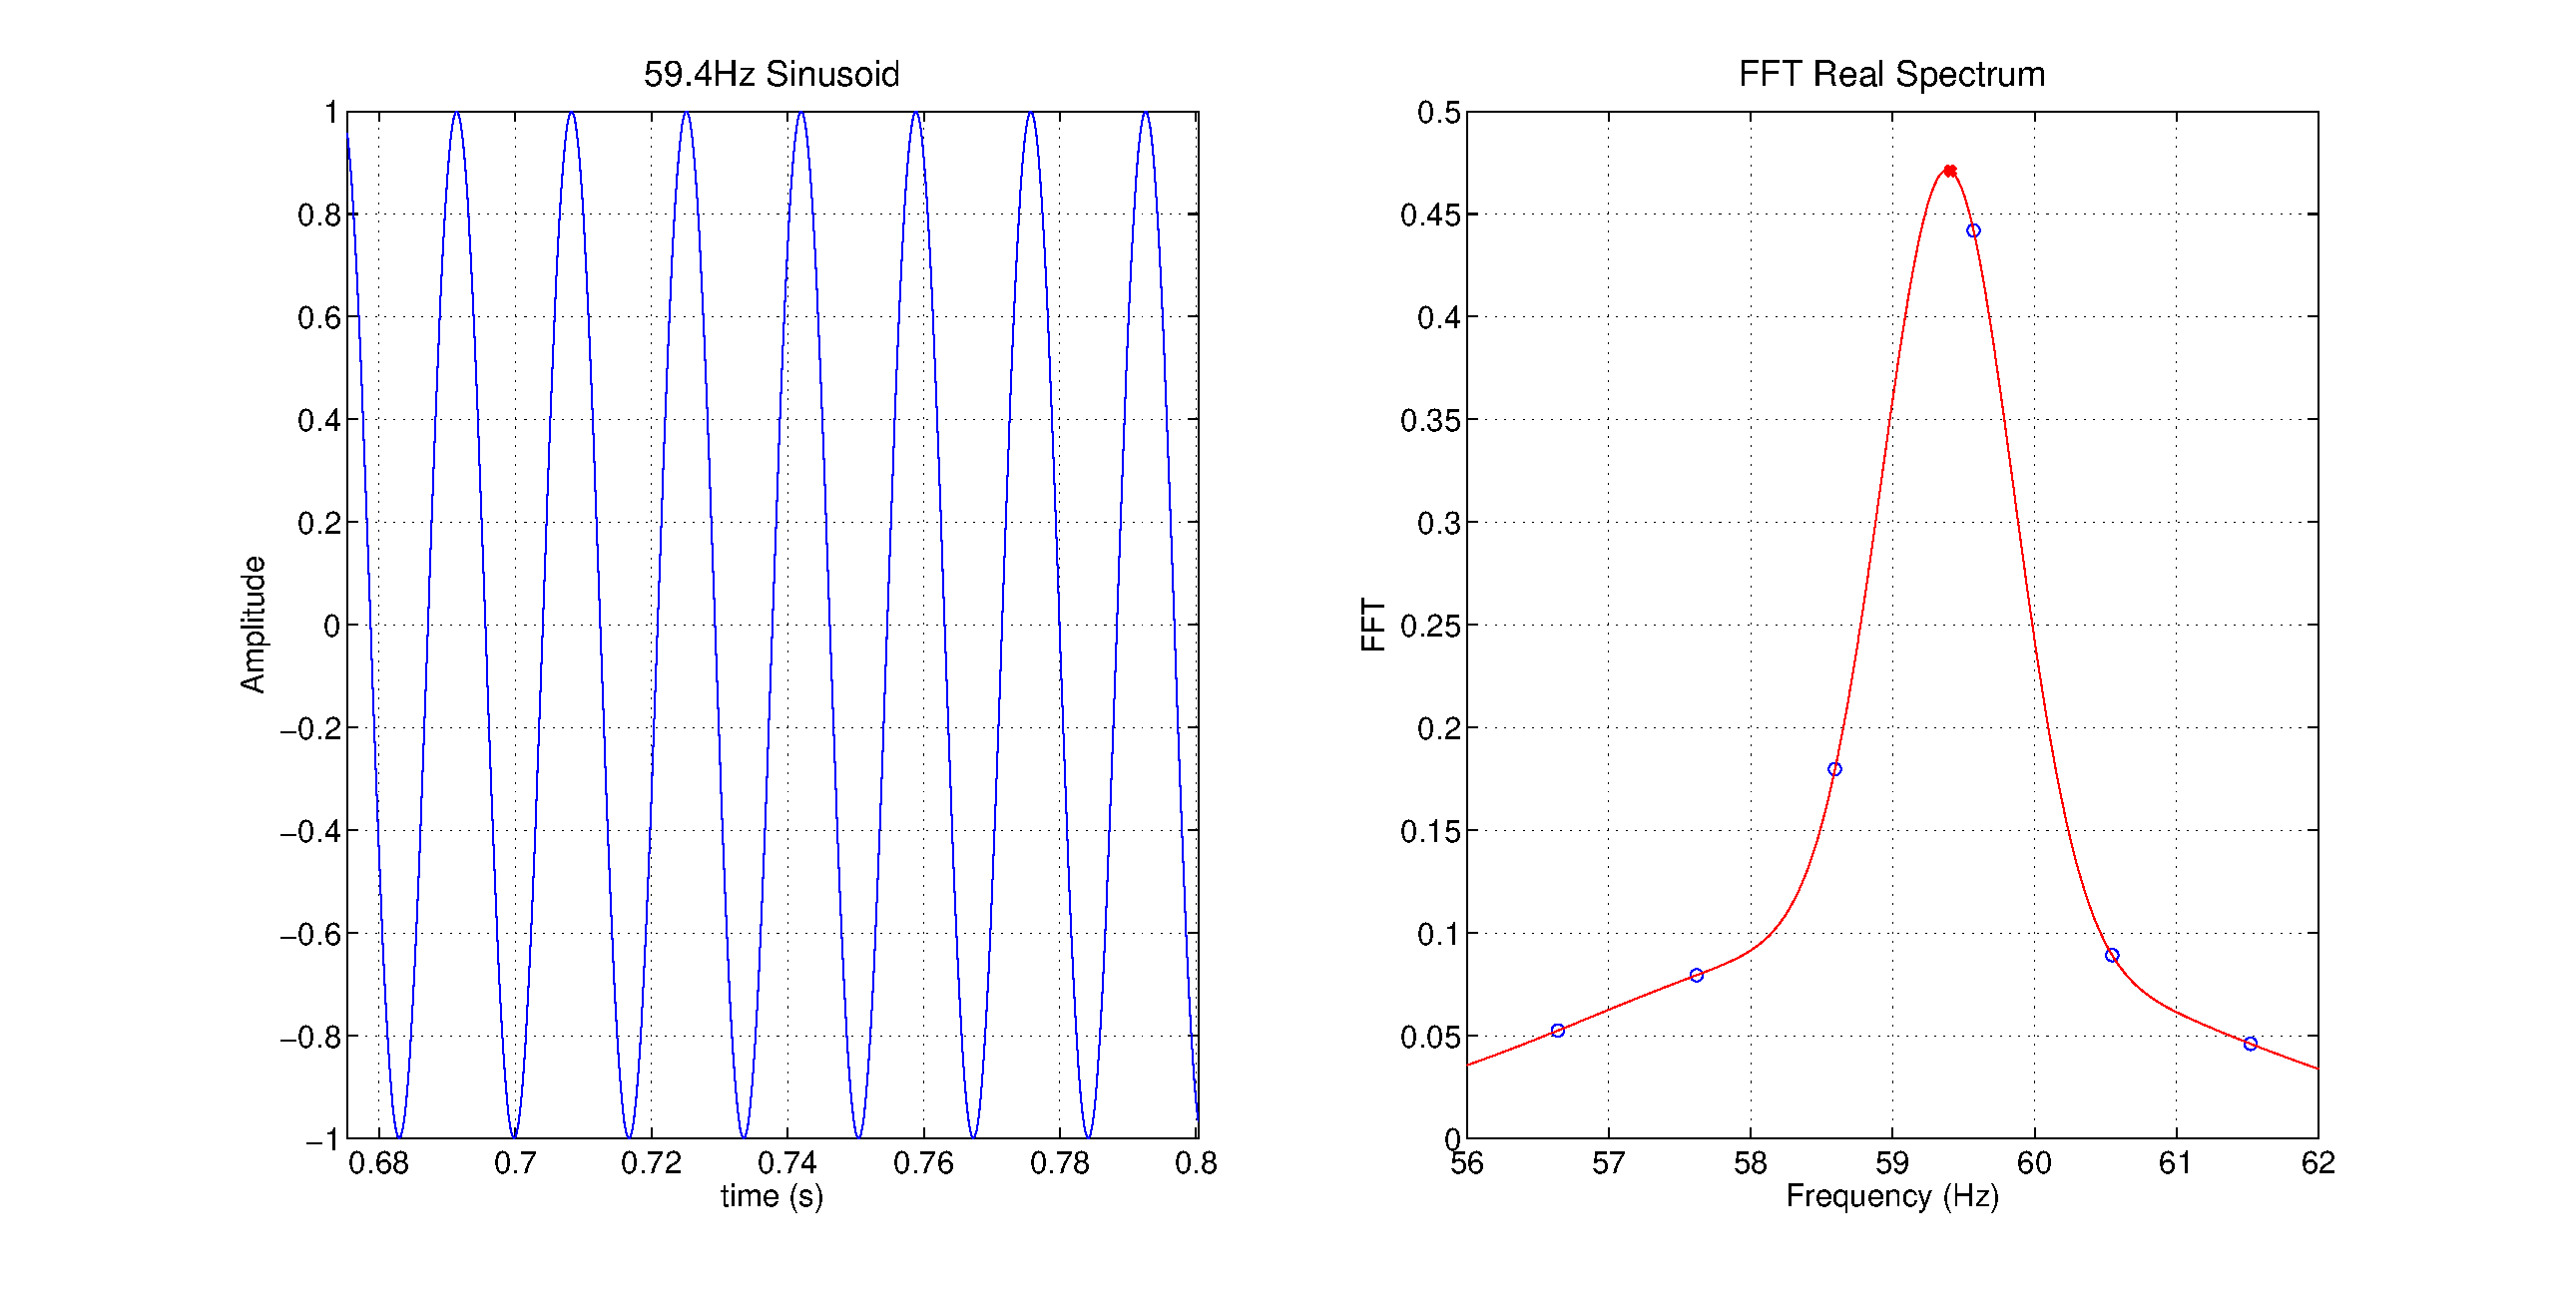
\includegraphics[width=0.9\textwidth]{img/fftFit.eps}
\end{center}
\caption{Calculating the fundamental frequency using FFT and peak fitting.}
\begin{center}
\textit{Left:} 59.4Hz sinusoid. \textit{Right:} Gaussian fit to the 6 point stradeling the peak. Extracted maximum is $59.39Hz$.
\end{center}
\end{figure}


Every window recorded passes through the first three steps in OPQBox1 analysis system. However, only windows with frequency and voltage outside the threshold are sent to aggregation.  The filter task checks the computed values against the tolerances and selects windows to send to the cloud. We defined our thresholds to be:

\begin{itemize}
\item $\pm 0.5Hz$ deviation from the $60Hz$ norm.
\item $\pm 7V_{rms}$ deviation from the $120V_{rms}$ norm.
\end{itemize}

The windows selected by the filter task are considered events and are prepared to be sent to the aggregation service via a WIFI dongle. The window is serialized into JSON, along with the appropriate metadata, and sent over a websocket connection to the aggregation server. Additionally, the OPQBox1 sends a measurement packet every 15 seconds. This packet does not contain the raw waveform, instead sending only the utility frequency, $V_{rms}$ and a timestamp of a window. This allows us to monitor the voltage and frequency trends even during the normal power grid conditions. 

\subsection{Aggregation Infrastructure}
The Open Power Quality aggregation software, titled OPQHub, is responsible for communicating with the OPQBox devices, and serving user side content. It is written in Java using the Play framework. OPQHub provides a rich visualization suite, along with a data querying API for developers. The description of OPQHub is beyond the scope of this paper. A white paper on this topic has been previously published by OPQ.\ref{tony}

\section{Results}

In this section we discuss the preliminary results of  OPQBox deployment. First we present the daily trends seen by our network. Next we correlate the voltage trends to the output
of a PV installation. Finally we take a look at an event recorder on two geographically separated devices.

\subsection{Daily Trends}

Using our power quality sensor network, we are able to monitor daily trends throughout the grid. Figure \ref{fig:trends} shows a typical daily trend for three devices. This data was 
collected on Oct 26. The ``CSDL'' device was located in the Collaborative Software Development Lab at the University of Hawaii. The ``Justin'' device was located in the high-rise apartment, near
downtown Honolulu. Finally, the ``Philip'' device is located in a residential home with a rooftop PV installation in Kailua.

\newpage
\begin{figure}[h!]
\centering
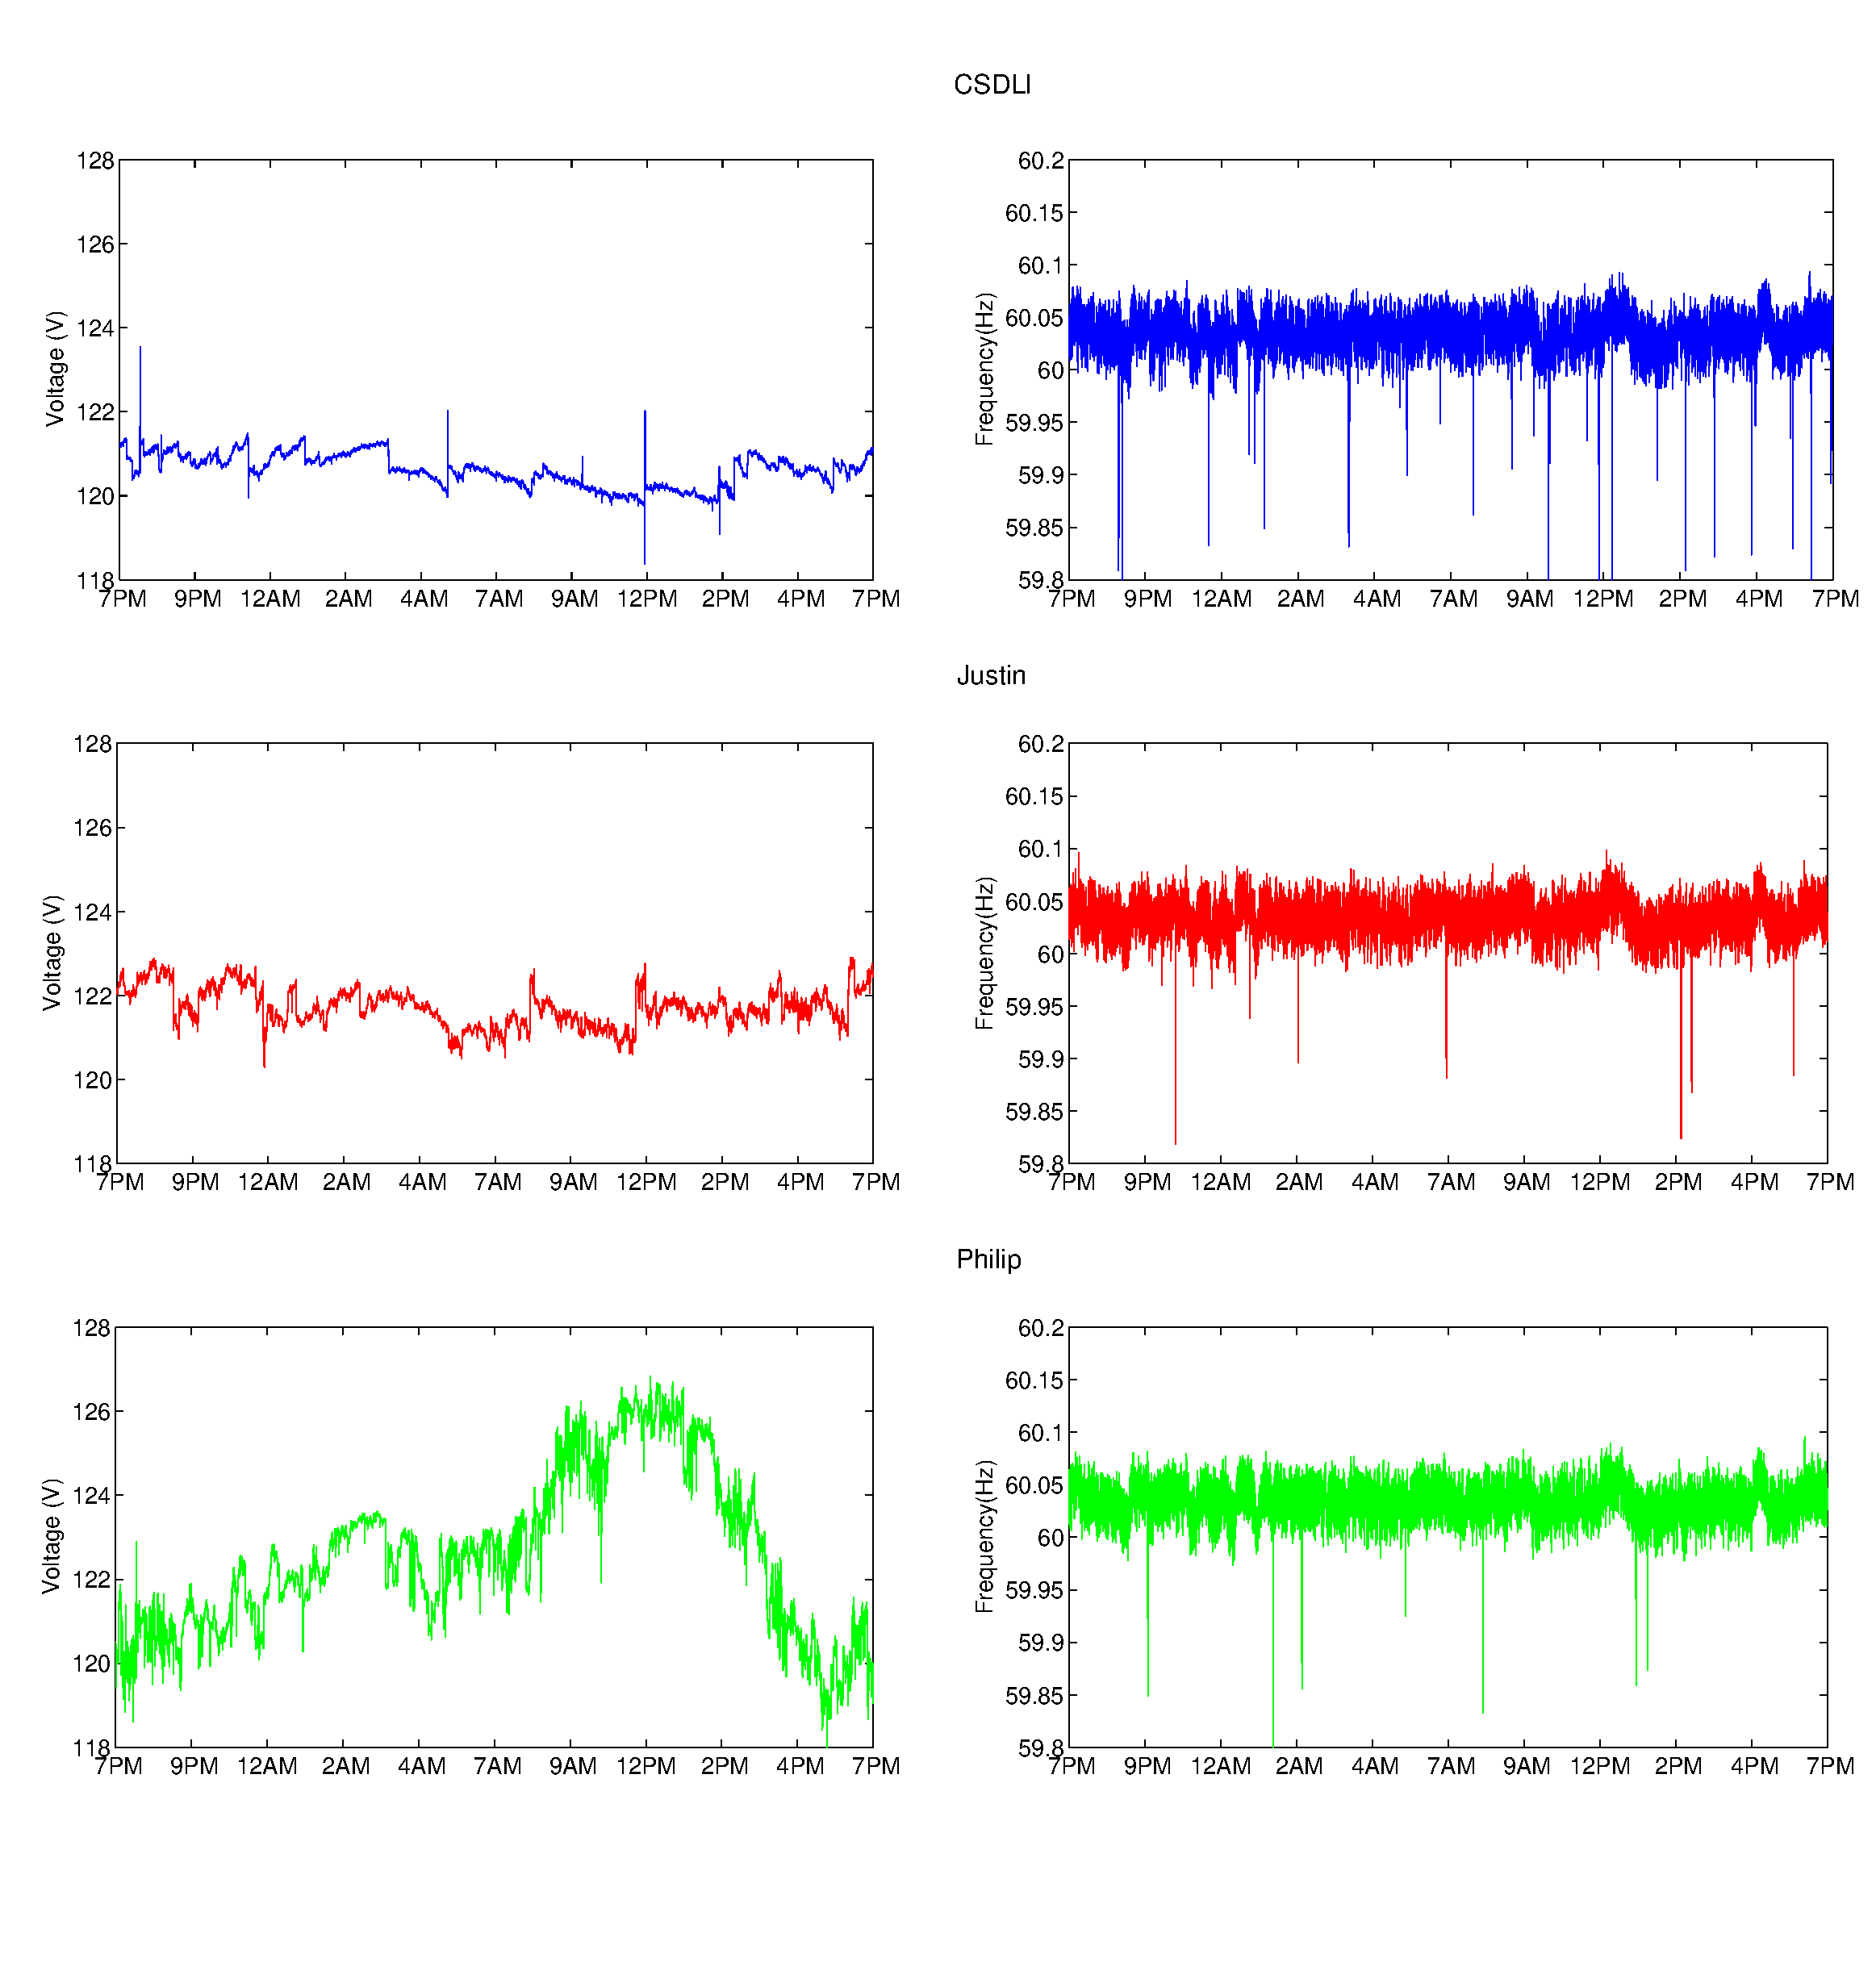
\includegraphics[width=\textwidth]{img/1Day.eps}
\caption{Voltage and frequency readings for three devices over Oct 26.}
\label{fig:trends}
\end{figure}
\newpage

The frequency measurements track each other throughout the day. This is to be expected since grid frequency is set by a few central generators. Voltage data recorded by the CSDL and  Justin devices show the same behavior throughout the day, however local voltage disturbances dominate the short term trends. In the case of the Philip device, however, a daily voltage fluctuation of $~10V_{rms}$ was observed daily. We attempt to explain this phenomenon by correlating the voltage reading to PV activity in the section \ref{sub:PV}.

\subsection{Grid Voltage and Grid Tied Photovoltaic Installations}
\label{sub:PV}
The top graph in Figure \ref{fig:samehouse} shows the RMS voltage recorded from August 1 to August 8 for the ``Philip'' device in a residential home in Kailua, Oahu. The bottom plot shows the power produced by 
a grid tied PV installation, located on the roof of the same house.

\begin{figure}[h!]
\centering
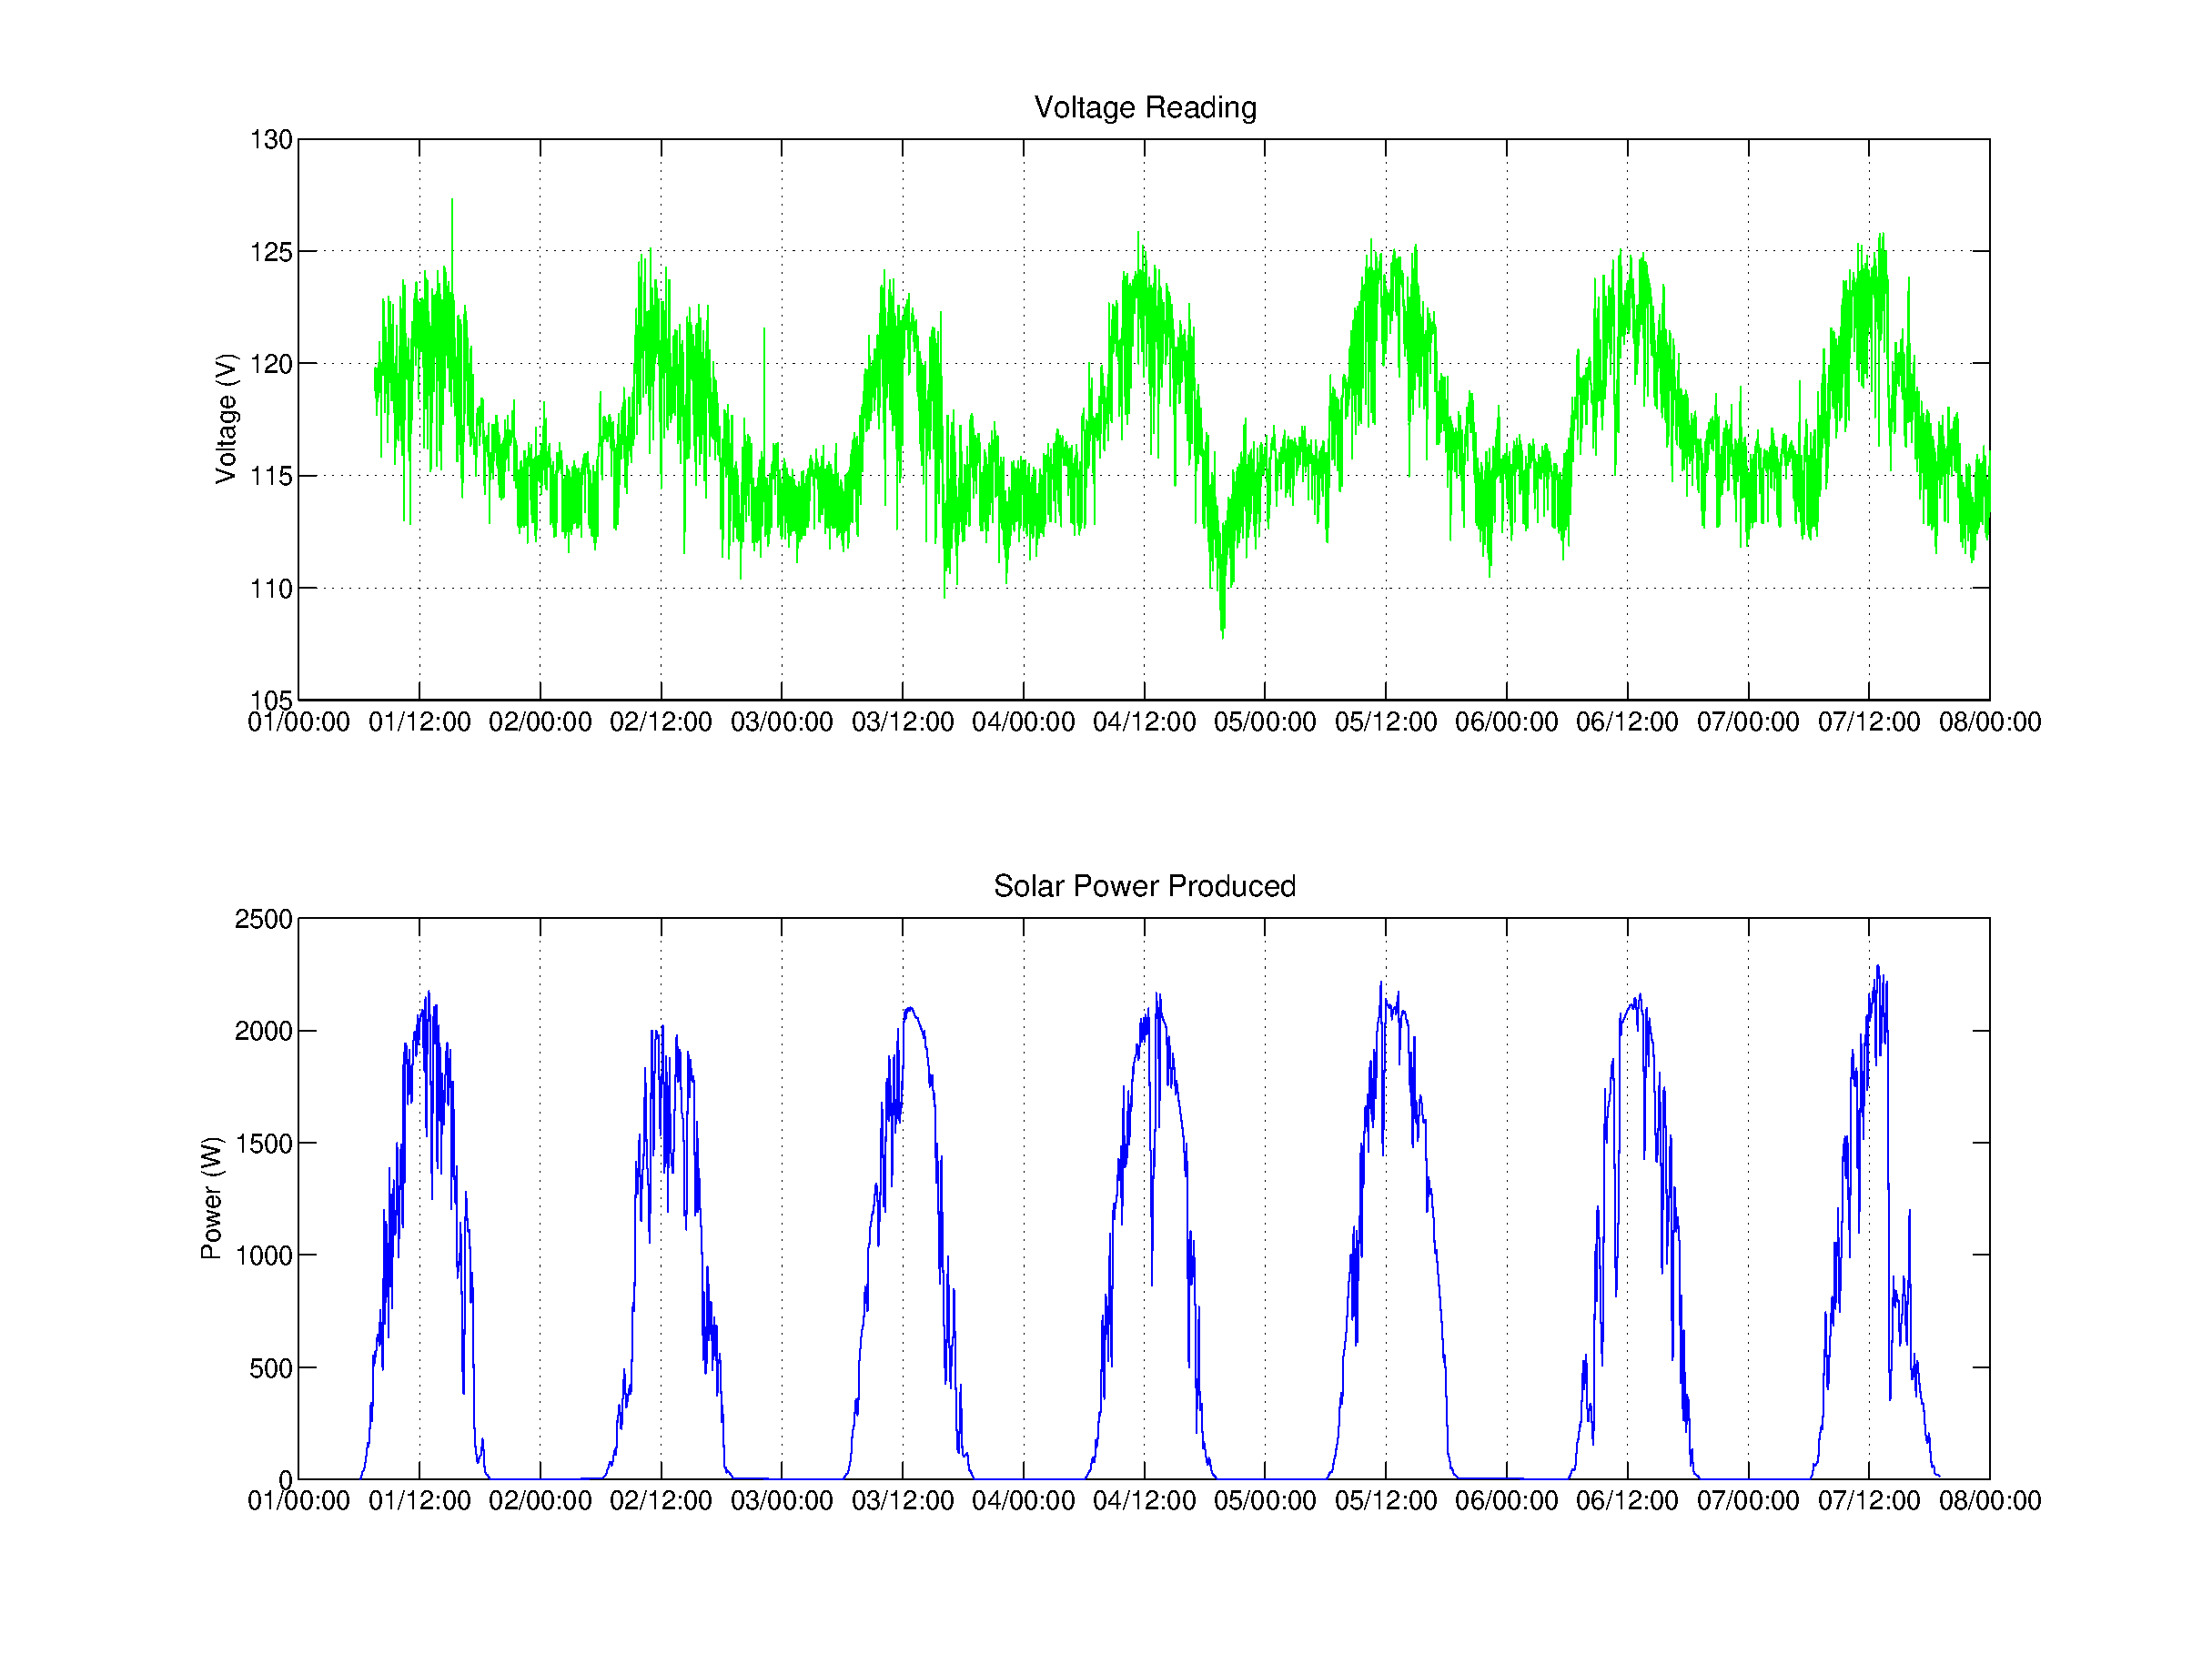
\includegraphics[width=\textwidth]{img/solarCorelationSameHouse.eps}
\caption{Grid voltage and solar power produced. Device and PV located in the same house.}
\label{fig:samehouse}
\end{figure}

The correlations between the power produced and the voltage are clearly shown in Figure  \ref{fig:samehouse}. Some of the more fine-scale correlations are also visible. 
For example, a large drop in PV output on August 4 13:00pm is correlated to a drop in the utility voltage. This leads us to believe that solar panels contribute to the
variation of the line voltage of the house they are supplying. This effect has been demonstrated locally in the past.\cite{pq_effect1} This begs the question: how do photovoltaics influence the grid voltage as a whole?

\begin{figure}[h!]
\centering
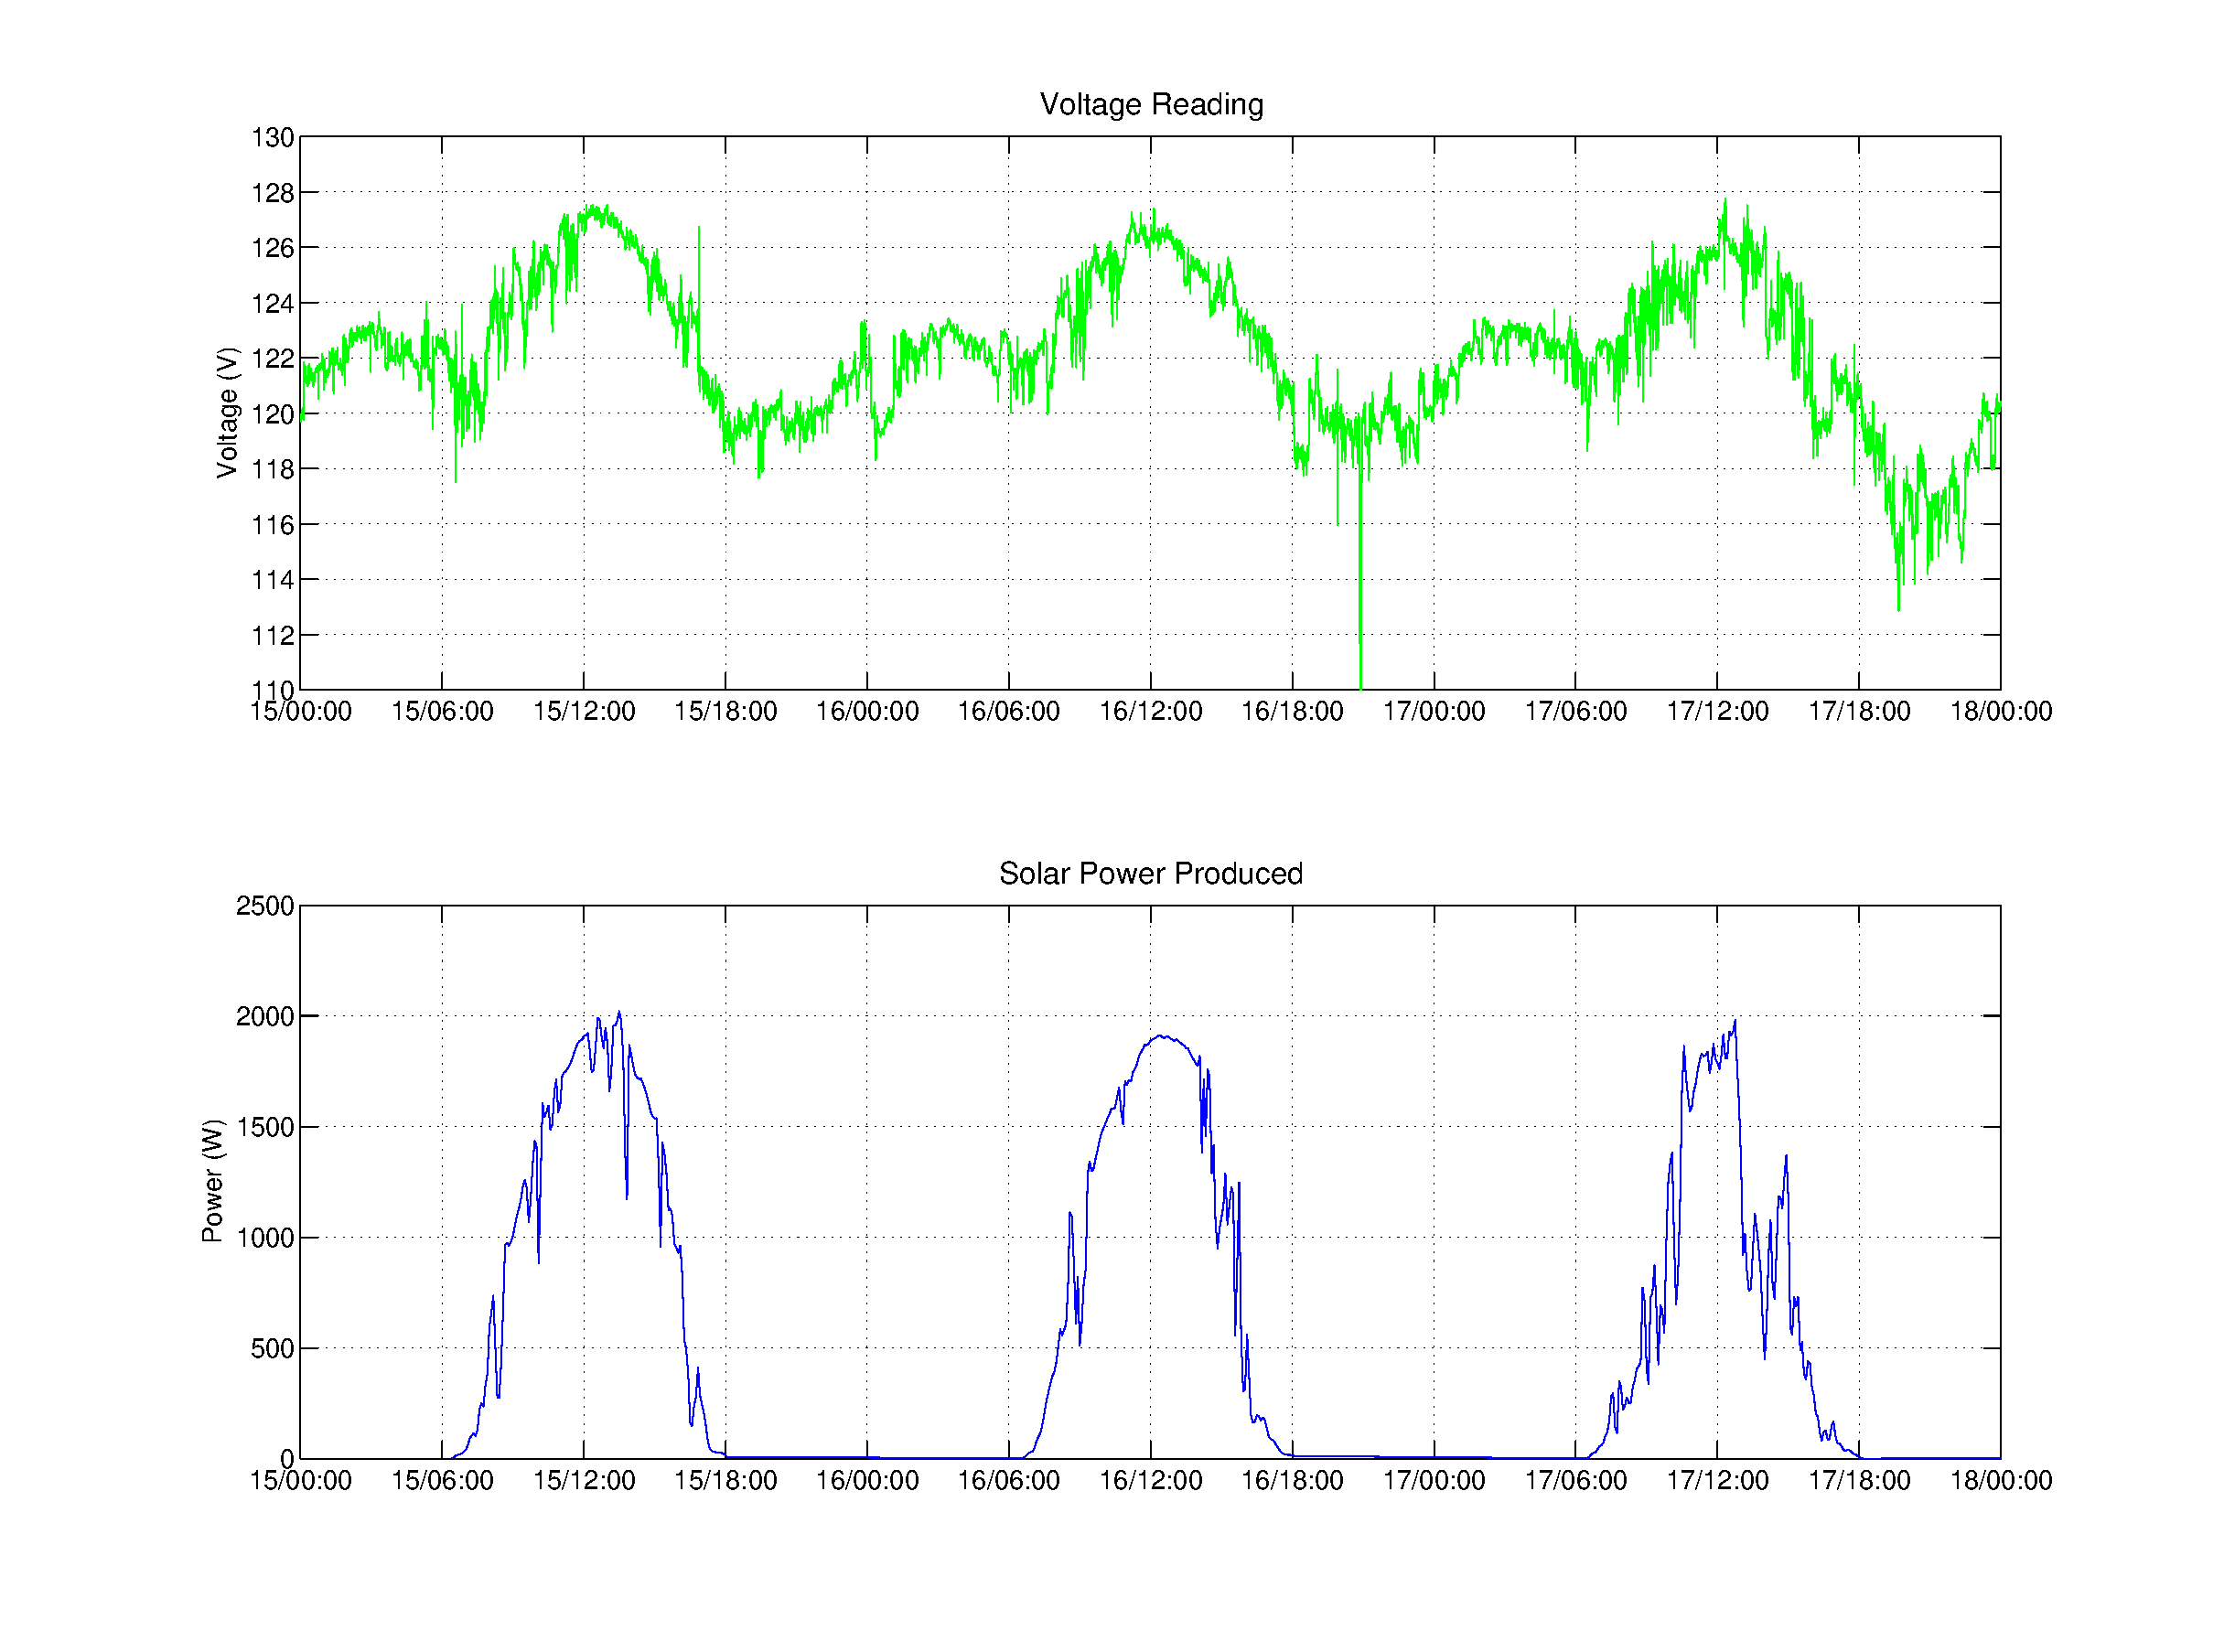
\includegraphics[width=\textwidth]{img/SunnyWeather.eps}
\caption{Grid voltage and solar power produced. Device and PV located are separated by ~20 miles.}
\label{fig:diffhouse}
\end{figure} 

Figure 3.2 shows the same graphs as Figure \ref{fig:samehouse} for October 15 to October 18. This time, however, the OPQBox1 device and the PV unit are separated by 20 miles. The house containing the OPQBox1 did not have a grid tied PV system. Correlations are present nonetheless; the line voltage measured by the device is proportional to the power generated by the PV installation. A possible explanation for this effect is that PV installations affect the line voltage across the whole grid. Oct 15-17 were clear days with minimal cloud cover, which implied that PV installations were generating power across the island, perhaps affecting the grid voltage while doing so. One way to answer this question is examine the line voltage trend while the PV installations
across the island are idle. 

On the days of October 17 through October 19, Hurricane Ana passed within 100 miles of the island of Oahu. Its passing brought heavy clouds which enveloped the entire island. Clouds began to form late afternoon Friday, October 18, as demonstrated by the power generation drop in figure \ref{fig:diffhouse} along with the line voltage drop recorded by the device. Voltage and Power readings for October 18 through October 20 are shown in figure \ref{fig:storm}.

\begin{figure}[h!]
\centering
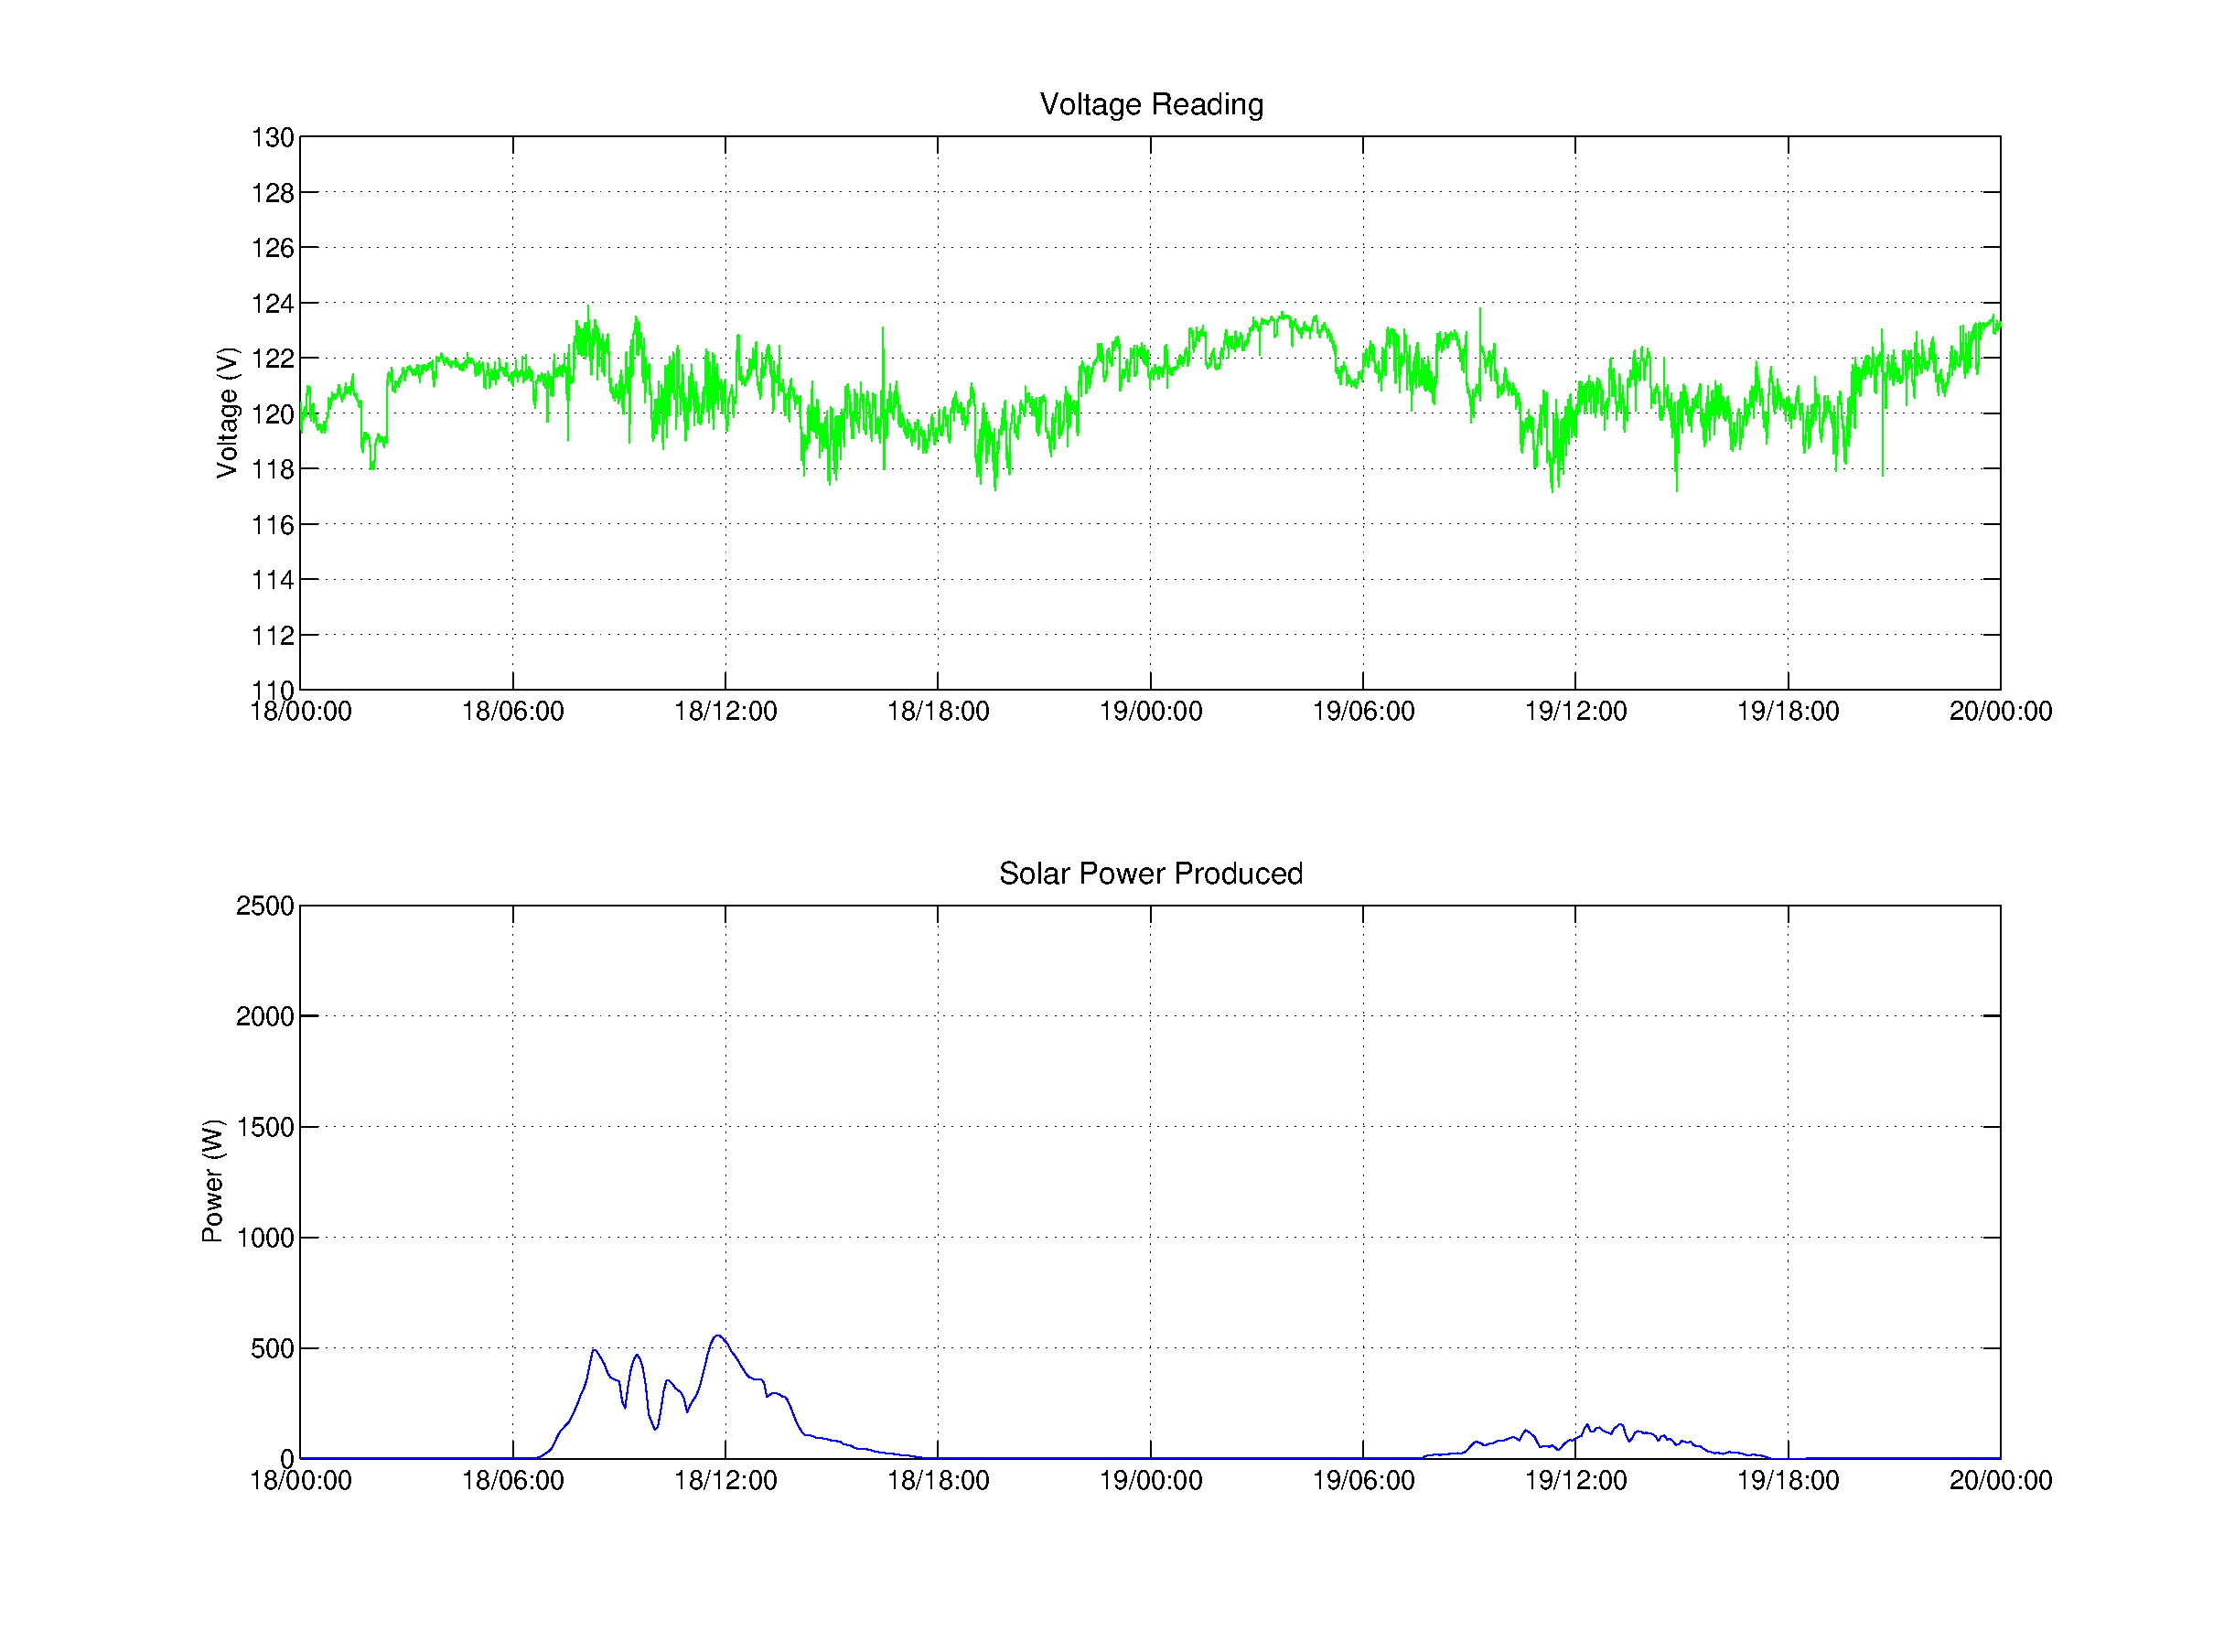
\includegraphics[width=\textwidth]{img/Stormy.eps}
\caption{Grid voltage and solar power produced during hurricane Ana. Device and PV located are separated by ~20 miles.}
\label{fig:storm}
\end{figure} 

As shown in Figure \ref{fig:diffhouse}, during peak hours, the PV installation was generating 2kW of power, yet during the storm on October 18 and 19 it was generating 550W and 100W respectively. Furthermore the line voltage did not exhibit the same variations we saw in figure \ref{fig:samehouse} and figure \ref{fig:diffhouse}. While more research is required, the data we collected over the last several months provides some evidence that the high penetration of PV installations on Oahu affects grid voltage. 

\subsection{Grid Wide Events}

\begin{figure}[h!]
\centering
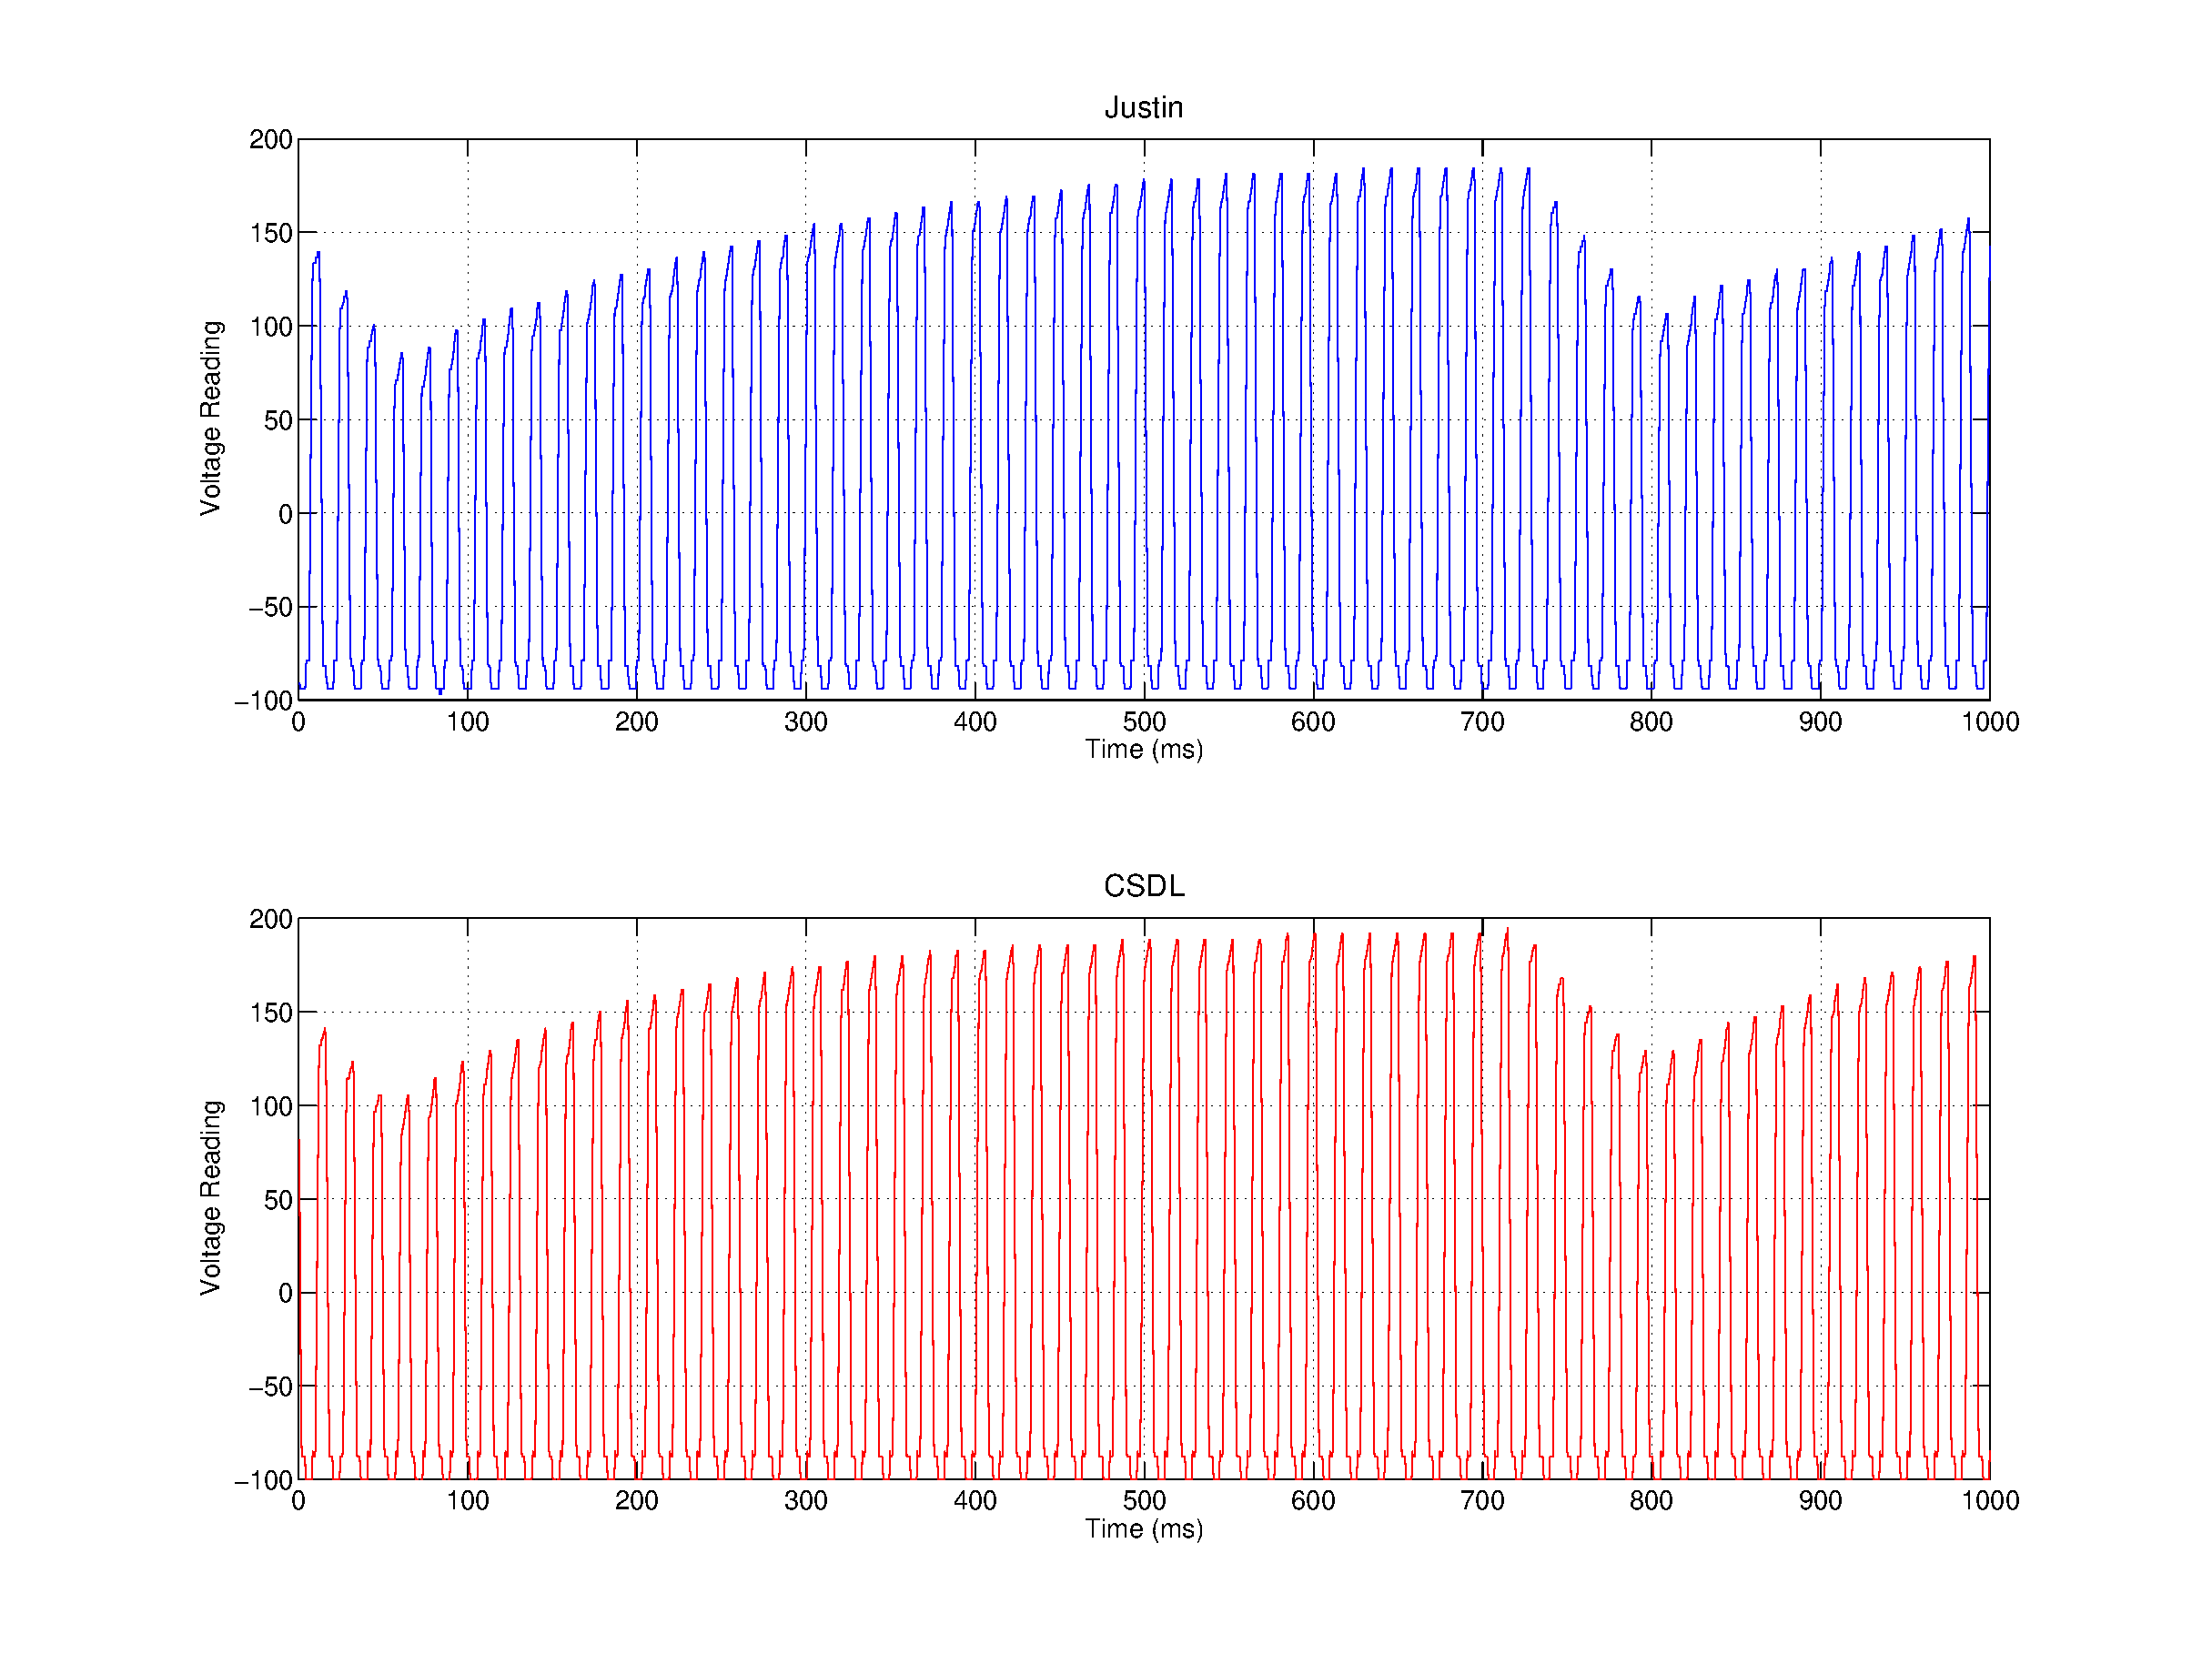
\includegraphics[width=\textwidth]{img/gridwide.eps}
\caption{Grid-wide event recorded by two devices on 13:46 on Sept 30. Devices are 10 miles apart.}
\label{fig:grid}
\end{figure} 

As described in Subsection 2.3, our system is able record both long term trends, and short term transients. Unfortunately only several of such transients have been confirmed to be grid wide. An example of such an event is shown in figure 3.4.

\begin{figure}[h!]
\centering
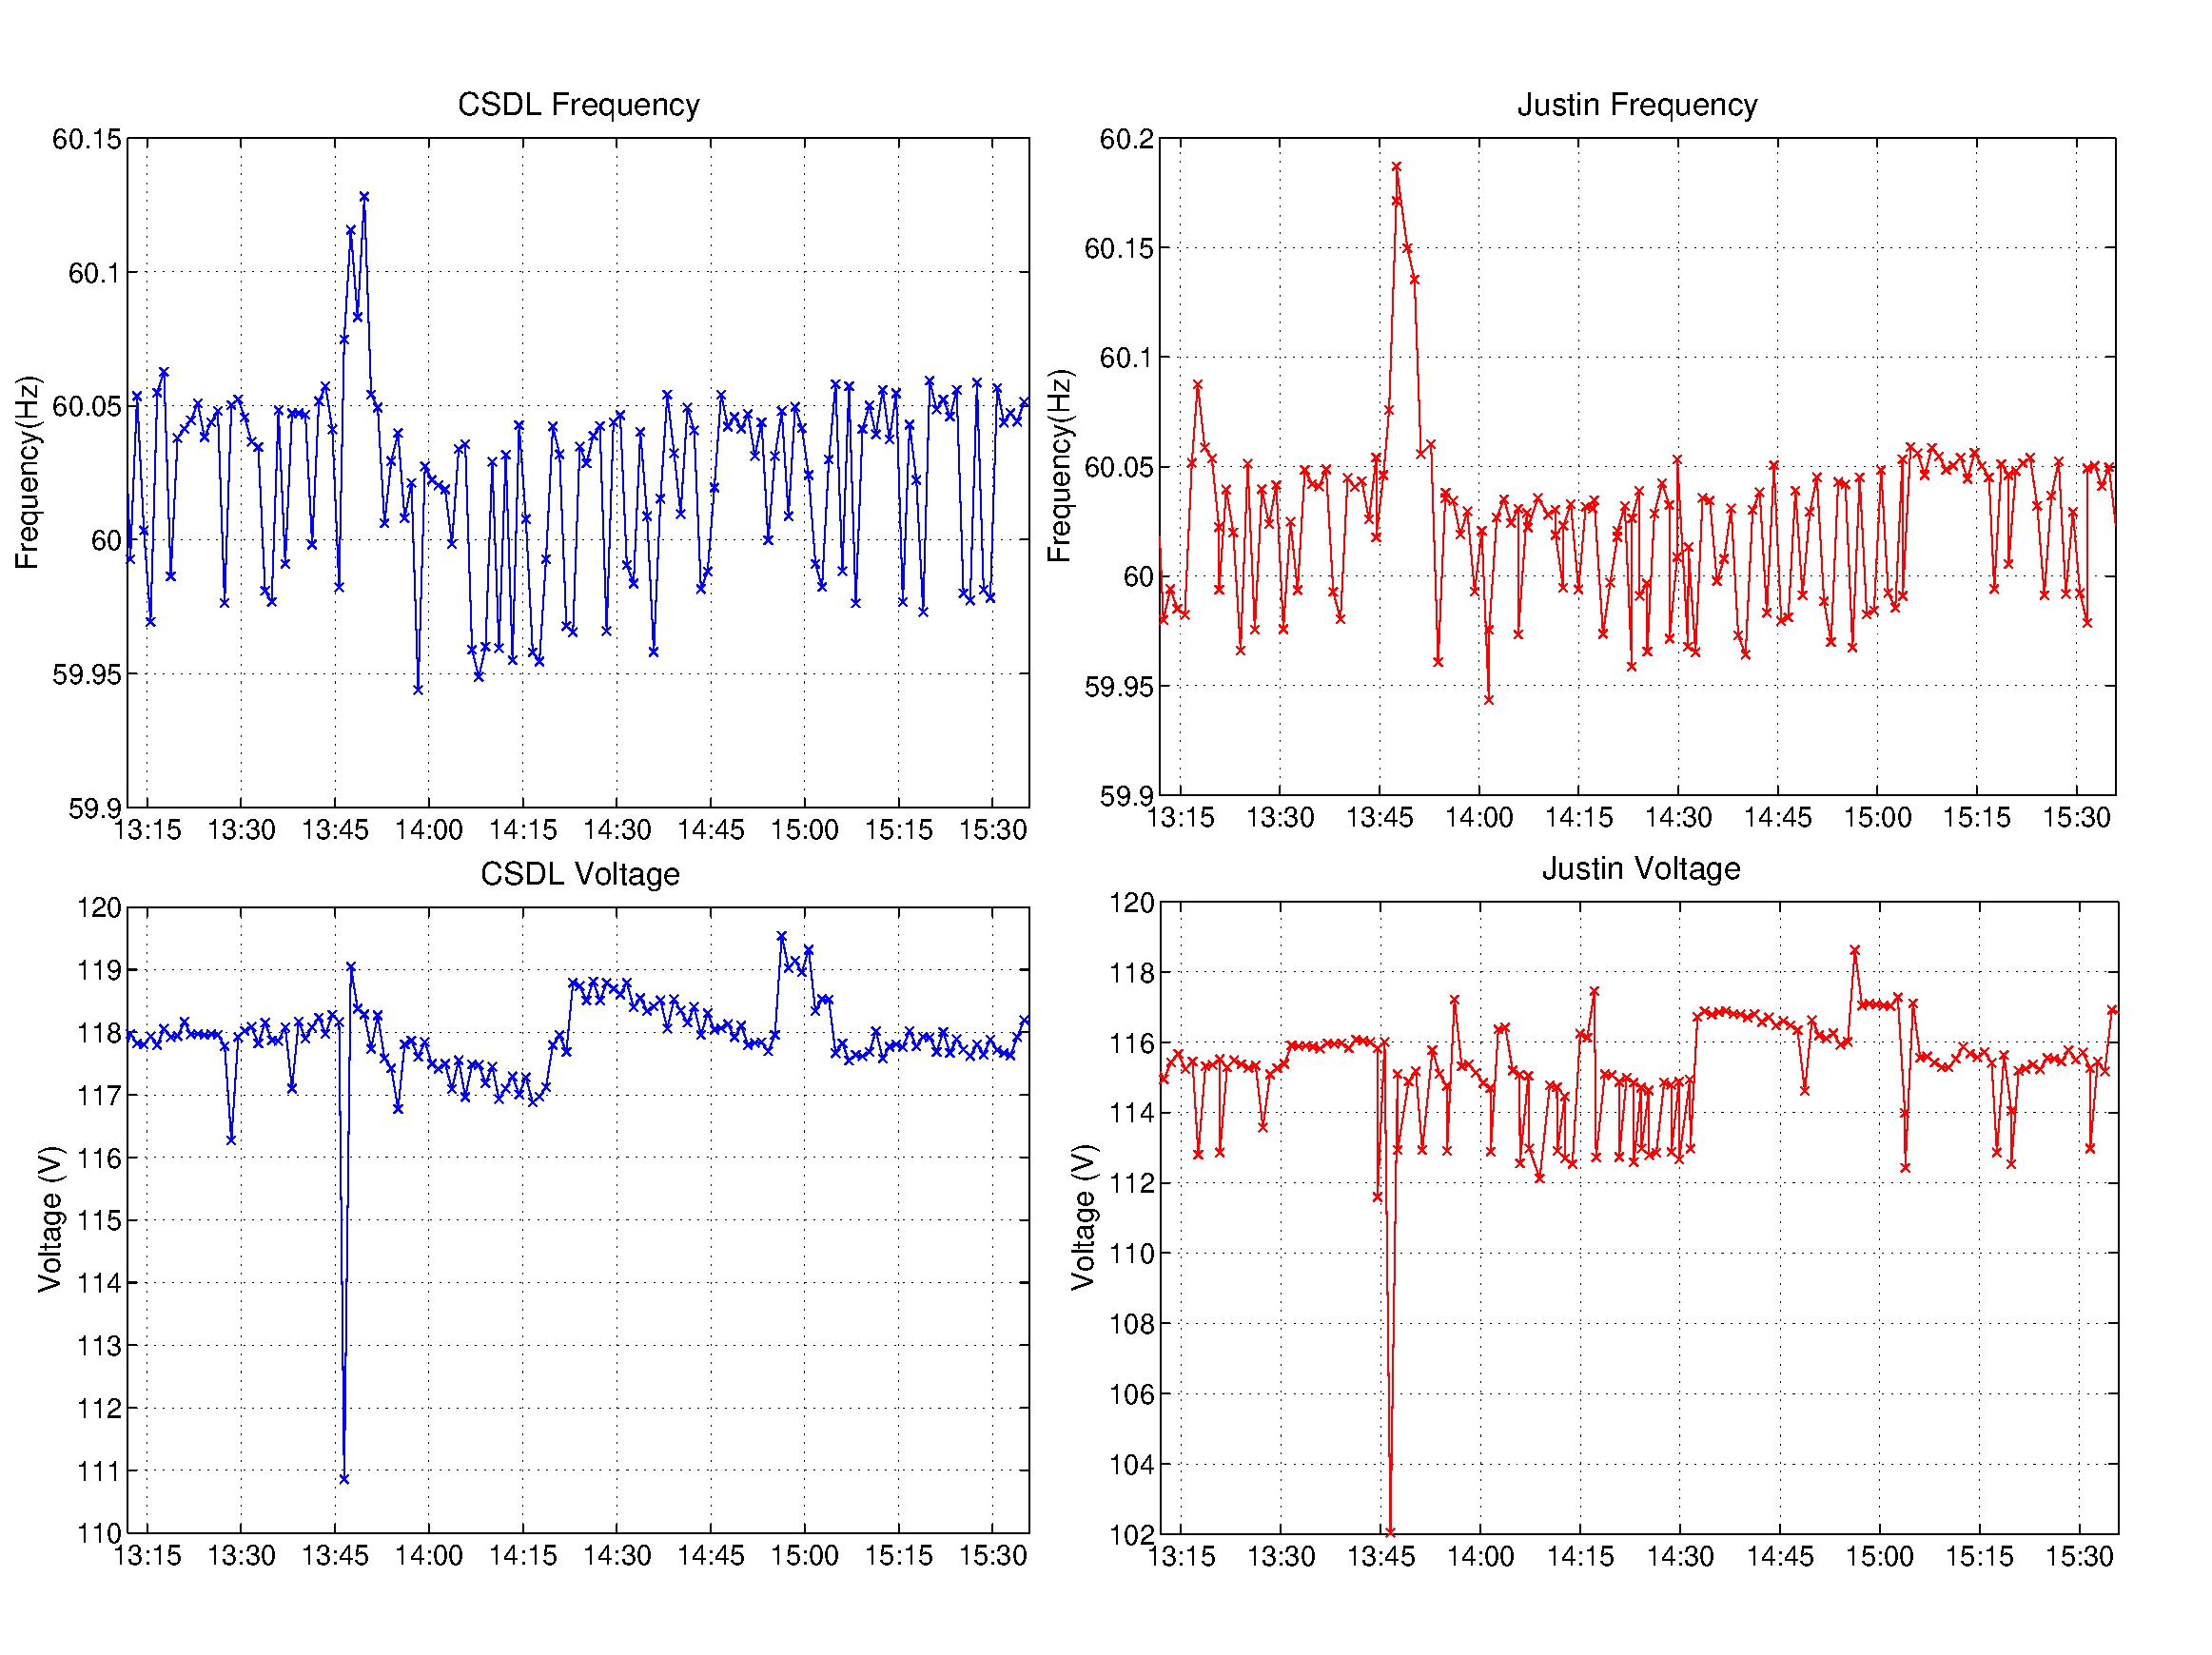
\includegraphics[width=1\textwidth]{img/gridwide_trends.eps}
\caption{Voltage and frequency trend for the event shown in Figure \ref{fig:grid}.}
\label{fig:daytrends}
\end{figure} 
The event above is two voltage sags lasting 6 cycles, separated by ~700ms. It was seen by two devices, one located at University of Hawaii at Manoa, and the other 10 miles away in a high rise apartment building. The timestamp between the two waveforms differed by 18ms, or approximately one grid cycle. Using the data we collected we are able to examine the the voltage and frequency trend around the event time as shown in figure \ref{fig:trends}.

Figure \ref{fig:daytrends} shows that while the voltage dip quickly recovered, frequency variations continued for several minutes. While the cause of this particular disruption will likely remain unknown, events such as this prove both the feasibility and the need for deployment of a power quality monitoring system such as OPQBox1 and OPQHub. We have shown in section \ref{sub:PV} that power quality is subject to environmental factors. As our technology matures, the detection, clustering, classification and analysis of grid-wide events will allow us to further correlate power quality disturbances to environmental data. This may in term support new forms of prediction and control.


\section{OPQBox2}\label{chap:further}

During the initial deployment of the OPQBox1 and OPQHub several problems have been discovered. In order to overcome these problems, the next generation of OPQbox is in active development.
The list of proposed  changes is shown Table \ref{tbl:comp}. 

\begin{table}[h!]
\caption{Comparison of OPQBox1 and OPQBox2}
\label{tbl:comp}
\begin{tabular}{|l|l|l|}
\hline
\textbf{Feature}        & \textbf{OPQBox1}               & \textbf{OPQBox2}                     \\ \hline
Synchronization         & NTP/Software sampling    & NTP/Hardware sampling         				 	\\ \hline
Sampling rate           & 4kSps                 & Up to 50kSps Nominal 15.36kSps 					\\ \hline
Voltage sensing method  & Wall Wart transformer & Resistor Divider            					\\ \hline
Power Fault Handling    & NONE                  & FRAM waveform storage       					\\ \hline
Communication Capabiliy & UART                  & UART/SPI/USB/$I^2C$               					\\ \hline
On board processing     & NONE					& ARM CPU with FPU								\\ \hline
\end{tabular}
\end{table}

On board processing for OPQBox1 was performed by the Raspberry PI SBC. Raspberry PI was an attractive option, due to the wide range of interfaces, ample processing power and small
footprint. However due to the limitations imposed by the non-realtime nature of Linux, it became impossible to guarantee consistent timing between devices. Even with perfectly synchronized
clocks, an RMS jitter of up to 50ms was observed between window samples. OPQBox2 is based on a dedicated 32bit ARM MCU. This MCU is responsible for controlling
the sampling rate of the device, and since this process is interrupt driven, the scheduler jitter will be eliminated. Furthermore, the MCU is responsible implementing a 
phase locked loop such that a first and last sample of a grid cycle fall on the zero crossing. This will simplify the analysis and improve synchronization between devices.

Due to the window size used in OPQbox1,  it was almost impossible to detect short-lived transients. In order to improve transient detection, OPQBox2 will analyze the input one grid cycle 
at a time, thereby shrinking the window from 1s to 16ms. This will require a new algorithm for frequency extraction, however, since OPQBox2 includes a dedicated CPU/FPU this analysis will be performed by the realtime controller. Fitting is being considered as an algorithm of choice, since it will provide phase, amplitude and fundamental frequency information.

Sampling rate increase in OPQBox2 is dictated by the IEEE Std 1159.\cite{ieee_pq} This standard recommends a minimum of 256 points per grid cycle, or a sampling rate of 15.36kSps. In order to accomplish this
the MSP430AFE is replaced by a dedicated 50kSps ADC. However during our calibration of the OPQBox1 we found that the wall-wart transformers used in sampling had on average 3kHz of bandwidth.
In order to catch short lived transients and justify the high sampling rate, the transformer was removed from the OPQBox2 design. Instead voltage scening is performed via a simple resistor
divider, and an isolation amplifier. OPQBox2 leaves a large margin of conversion rate for future applications, and sampling rate of 800 samples per grid cycle can be achieved if required.

During development of OPQBox1 we focused on UART as primary method of communication with the outside world. Raspberry Pi provided all the processing and WIFI for communication. OPQBox2 on the other hand provides several possible interfaces, and since the processing is performed on the device, any communication controller compatible with the SPI UART or $I^2C$
can be employed. This allows us to tailor OPQBox2 to operate independent of the communication interface, thus allowing us to monitor power quality in locations inaccessible to WIFI.

Power outages have not been considered in the design of OPQBox1. Since data leading up to the power outage can provide insight into the nature and the cause of the fault, OPQBox2 was
designed to handle outages. Battery and supercapacitor have been considered during the design stage, however they added bulk and did not necessarily preserve the data during a long term power failure. Instead OPQBox2 design uses ferromagnetic RAM to buffer at most 30 grid cycles of high resolution waveforms. Since FRAM maintains it state during a power interruption, 
OPQBox2 is able to provide 500ms worth of high resolution voltage waveforms leading up to the outage.

\section{Conclusions}

As the grid evolves, so must its monitoring capability. OPQHub and OPQBox represent a first step in our effort to develop a scalable, accurate, and open power quality sensor network. Through the data collected via the OPQ network, we are able to get a glimpse of the problems facing the Oahu grid. Furthermore, Oahu represents a possible future of the US mainland power generation system. As the penetration of consumer renewable energy generators increases throughout the world, power grids must adapt.  Utility companies generally do not monitor the power grid state below the substation level, because traditionally residences and businesses were considered consumers. We have shown that this may create a potentially dangerous situations for neighborhoods with high penetration of renewable resources. As our technology matures and our network grows in number of sensors and precision, more patterns will undoubtedly emerge. Our end goal is to provide utilities, consumers and researchers with an open system, and open data for monitoring power grids.

\newpage
%%% Switch to appendix mode
\appendix

%%% Bring in any appendices from external file
%%%%%%%%%%%%%%%%%%%%%%%%%%%%%% -*- Mode: Latex -*- %%%%%%%%%%%%%%%%%%%%%%%%%%%%
%% uhtest-appendix.tex -- 
%% Author          : Robert Brewer
%% Created On      : Fri Oct  2 16:31:12 1998
%% Last Modified By: Robert Brewer
%% Last Modified On: Mon Oct  5 14:41:05 1998
%% RCS: $Id: uhtest-appendix.tex,v 1.1 1998/10/06 02:07:03 rbrewer Exp $
%%%%%%%%%%%%%%%%%%%%%%%%%%%%%%%%%%%%%%%%%%%%%%%%%%%%%%%%%%%%%%%%%%%%%%%%%%%%%%%
%%   Copyright (C) 1998 Robert Brewer
%%%%%%%%%%%%%%%%%%%%%%%%%%%%%%%%%%%%%%%%%%%%%%%%%%%%%%%%%%%%%%%%%%%%%%%%%%%%%%%
%% 

\section{Gen 1 Schematics}


%% Just for demo purposes, include all entries from bib file
\nocite{*}

%%% Input file for bibliography
\bibliography{thesis}
%% Use this for an alphabetically organized bibliography
\bibliographystyle{plain}
% Use this for a reference order organized bibliography
%\bibliographystyle{unsrt}

\end{document}
